%%%%%% USE PDFLATEX !!! %%%%%
%% CMD pdflatex -synctex=1 -shell-escape -interaction=nonstopmode %.tex %%
\documentclass[a4paper, 11pt,twoside=true,UTF8]{scrartcl}
\usepackage{ctex}
\usepackage{geometry}
\usepackage[table,xcdraw]{xcolor}
\usepackage{Rapport2CN}
\usepackage{enumitem}
\usepackage{lipsum}
\usepackage{listings}
\usepackage{enumitem}
\usepackage{minted}
\renewcommand{\figurename}{图}
\renewcommand{\tablename}{表}

\newcommand{\dts}{$\vcenter{\hbox{\tiny$\bullet$}}$}
\graphicspath{{./}{./img/}{./fig/}{./image/}{./figure/}{./picture/}
	{./imgs/}{./figs/}{./images/}{./figures/}{./pictures/}}

%%% Paramètres pour les footers et la page de titre
\newcommand{\lab}{数据科学导论课程报告}
\newcommand{\tit}{数据科学之我见及其在疾病传播中的应用}
\newcommand{\nom}{NORM}
\newcommand{\superv}{Superviseur}
\newcommand{\depa}{计算机科学与技术}
\newcommand{\ID}{
	222019321102021\\
}
\author{
	刘锴睿\\
}
\newcommand{\names}{
	刘锴睿\\
}
\automark[section]{section}

\lehead*{%
  \makebox[0pt][r]{
    \colorbox{rahmen}{\makebox[\textwidth][r]{\bfseries\color{white}{\pagemark/\pageref*{LastPage}}\enskip}}\hspace*{1em}}%
  \headmark\hspace*{1em}\headrulefill%
}
\rohead*{%
  \headrulefill\hspace*{1em}\headmark%
  \makebox[0pt][l]{%
    \hspace*{1em}\colorbox{rahmen}{\makebox[\textwidth][l]{\enskip\bfseries\color{white}{\pagemark/\pageref*{LastPage}}}}}%
}
\lefoot{\color{darkgray}\small  2020年6月23日}
\rofoot{\color{darkgray}\small  2020年6月23日}
\cefoot{\color{darkgray}\small \itshape \tit\unskip\strut}
\cofoot{\color{darkgray}\small \itshape \qquad \qquad \tit\unskip\strut}
%%%%%%%%%%%%%%not????
\refoot{\color{darkgray}\small 数据科学导论课程报告\unskip\strut}
\lofoot{\color{darkgray}\small 2019 计算机科学与技术 01班\unskip\strut}

\addtokomafont{pagenumber}{\bfseries\color{white}}
\newcommand\headrulefill{\leaders\hrule width 0pt height 3pt depth -2.8pt \hfill}

%\renewcommand\titlepagestyle{empty}

\hfuzz 100pt
\hbadness 10000
\hfuzz 100pt
\hbadness 10000

% Inversion des espaces des marges

\let\tempmargin\oddsidemargin
\let\oddsidemargin\evensidemargin
\let\evensidemargin\tempmargin
\reversemarginpar

\sisetup{detect-weight=true, detect-family=true}

\renewcommand*{\maketitle}{%
\begin{titlepage}
\raggedleft
\includegraphics[scale=0.5]{sect_physique_pant}

\begin{center}
\horrule{0.5pt} \\[0.4cm] \vspace{-1.5ex}\textcolor{darkblue}
	 { \huge \bfseries \lab \\ \vspace{0.4cm} \tit }\\[0.1cm]\horrule{2pt} \vspace{-4ex}
%\horrule{0.5pt} \\[0.4cm] \vspace{-1.5ex}\textcolor{darkblue}
%	 { \huge \bfseries \lab \\ \vspace{0.4cm} \tit }\\[0.1cm]\horrule{2pt} \vspace{-2ex}
\end{center}
\vspace{1cm}
\begin{center}
 \textsc{\LARGE 西南大学\\ \large 计算机与信息科学学院 软件学院 \\ \depa \\ 数据科学导论 \unskip\strut} \vspace{-3ex} \\	
% \textsc{\LARGE Southwest University\\ \large School of computer and information science, school of software \\ \depa\unskip\strut} \vspace{-1.5ex} \\	
\end{center}
\vspace{3cm}
\begin{minipage}[t]{0.5\textwidth}
	\begin{flushleft}
		{\large \textit{年级} \\ 2019\unskip\strut
		}
	\end{flushleft}
\end{minipage}%
%
\begin{minipage}[t]{0.5\textwidth}
	\begin{flushright}
		{\large \textit{学号} \\ \ID\unskip\strut}           
		\vspace*{0.2cm}
	\end{flushright}    
\end{minipage}%

\begin{minipage}[t]{0.5\textwidth}
	\begin{flushleft}
		{\large \textit{班级}\\ 计算机科学与技术 01班	\unskip\strut
		}
	\end{flushleft}
\end{minipage}%
%
\begin{minipage}[t]{0.5\textwidth}
	\begin{flushright}
		{\large \textit{姓名}\\ \names	\unskip\strut}           
		\vspace*{0.5cm}
	\end{flushright}    
\end{minipage}%

\vspace{3.5cm}
\begin{center}
\begin{minipage}[h]{\textwidth}
    \vfill
    \begin{center}
        {\large 授课教师:陈怀东  \\ 2020年6月23日}
    \end{center}    
\end{minipage}%
\end{center}

\end{titlepage}
}

\begin{document}
\captionsetup[figure]{name={图},labelsep=period}
\captionsetup[table]{name={表},labelsep=period}
%%%%TITRE
%\newgeometry{left=3.8cm,right=2.5cm,bottom=0cm}
\renewcommand{\contentsname}{目录}
\renewcommand\refname{参考文献}
\newgeometry{left=2.8cm,right=2.8cm,bottom=0cm}
%\newgeometry{left=2.5cm,right=3.8cm,bottom=0cm}

\maketitle

\newpage
\section*{摘要}
\qquad \textit{数据科学是一门新兴的学科,它结合了统计学、数据分析、机器学习及其相关方法,旨在利用数据对实际现象进行“理解和分析”。简单来讲:数据科学是一门将数据变得有用的学科。在这篇报告中我将从我理解的数据科学说起,尝试使用数据集,对数据进行有限的分析并得到有趣且较为合理的结论}

\textit{在报告的第一部分,我阐述了我认为的数据科学,什么是数据科学。作为一个新兴学科,数据科学包含了那些学科的知识,在大数据的时代中数据科学在各个领域的应用;作为一个蓬勃发展的学科,数据科学有什么新技术;作为刚刚萌芽的学科,科学家与数据科学遇到了什么挑战,未来数据科学的发展前景。}

\textit{在报告的第二部分,我尝试访问data.gov与data.govt.nz,试图寻找我感兴趣且有效的数据集,并尝试将他们下载并分析他们,我下载了新西兰在1948至2011年间由于癌症去世的人的发病部位统计表,以及2008-2017年每日新西兰各城市PM2.5浓度数据,我将这个数据集导入R,使用ggplot对数据集进行了非常简单的数据可视化,却得到了很多令我意想不到的结果。之后,我讨论了数据公开的优缺点,对于我国政府在数据开放方面存在的问题进行了讨论,并将我国政府数据公开平台与较早使用数据开放平台国家的平台进行了对比,提出来一些切实可行的意见}

\textit{在报告的第三部分,我尝试对2020年4月19日COVID-19在全球传播数据进行分析,尝试使用R聚类与Q聚类结合主成分分析法得出了疾病全球大流行的量化定义,并通过使用响应面预测模型与基于COVID-19改进的SEIR模型在统计学与病毒传播动力学两个方向进行分析,得出了无症状感染者人数的预测模型,该模型具有较高的准确度}

\textit{在本学期数据科学导论的学习中,我不仅学到了如何使用R语言这个工具,更重要的是学到了如何科学的对已有的数据进行分析,用数据科学家的眼光审视问题,将生活中的问题与数学模型相结合以优化我们的决策}
\\ \\
\textbf{关键词:}\textit{数据科学;R语言;数据开放;聚类分析;主成分分析;响应面预测;修正 SEIR 模型;COVID-19}

\restoregeometry
% 修复溢出
\newgeometry{left=3.8cm,right=2.5cm,bottom=0cm}
\setcounter{page}{1}
\tableofcontents
\newpage
\newcounter{thispage}
\restoregeometry
%%%%%%% Début du document

\section{我对数据科学的认识与展望}
\subsection*{摘要}
\addcontentsline{toc}{subsection}{摘要}

\qquad \textit{21世纪是大数据和数据经济世纪,数据科学已成为一门新兴的热门学科,数据承载了丰富的信息,洞察力与潜力。 对数据的有机处理依赖于数据科学与大数据分析的新技术。很多人认为数据科学的火爆仅仅是因为有人炒作,数据科学尚处于发展的早期阶段,但挑战与机遇已经大量出现。数据科学是一门将现有统计学,数学理论有机结合起来,实现数据转化为对个人、组织和社会的价值的学科,这不仅在规模方面需要处理大量数据,在解决实际问题方面,也遇到了新的挑战。}

\textit{这一部分我阐述了数据科学的概述和前景,论述了我对数据科学应用与数据科学前景的看法。}
\\ \\
\textbf{关键词:}\textit{数据挖掘;数据科学;大数据;数据分析;计算信息学;数据经济;数据产业}

\subsection{什么是数据科学,数据科学包含什么}
\qquad “数据科学”一词在30年前就已存在,在1960年最初仅仅用作“计算机科学”的替代词。约15年后,该词用于定义不同领域中使用的数据处理方法应用的总称。 2001年,数据科学作为一门独立学科被引入。 《哈佛商业评论》在2012年发表文章称数据科学为“21世纪最有魅丽的学科”。

数据科学依靠大数据分析有意义的信息。数据科学及其二级学科结合了统计学与计算科学等不同的领域的知识,以发掘数据数据的价值并提供决策。

\textbf{数据科学包括数据挖掘,大数据和数据分析。}

数据挖掘是数据科学的主要分支。 数据挖掘致力于解决与海量数据或其中部分数据相关的问题。数据挖掘是在大型数据集中发现模式的过程,该模式涉及机器学习、统计学、数据库等多学科方法。 数据挖掘是计算机科学和统计学的一个跨学科子领域,其目标是从数据集中提取信息并将信息转换为易用的结构供进一步使用。 除了基本分析步骤外,它还涉及数据库管理、数据预处理、模型的推理、兴趣指标、复杂度分析,数据探索与可视化。

大数据是数据科学的另一个领域,涉及数据的处理分析,信息提取与处理传统方法无法处理的数据。在很多情况下,越大数据需要越大的算力,同时数据规模越大数据科学家越容易发现其中的错误。 大数据挑战包括数据获取、数据存储、数据分析、数据搜索、数据共享、数据传输、数据可视化、数据更新、信息隐私和数据源。 大数据与三个关键概念密切相关:数量、速度、种类。

数据分析是检查、清理、转换和建模的过程,目的是发现有用的信息,提供结论并支持决策。 数据分析具有多个方面和方法,涉及以不同领域的多种技术,并应用于商业,科学与社会科学领域。  在当今的商业世界中,数据分析在科学决策,帮助企业更有效地运作起着重要作用。

\subsection{数据科学的应用}
\qquad 随着数据科学的发展,数据科学已在越来越多的领域中得到广泛应用。 几乎所有学科的研究都依赖于大数据。 因此,数据科学在各个领域都有应用。

报告《分析、数据科学、机器学习的应用领域(2019):趋势与分析》中写道:客户关系管理与消费者分析,医疗保健,银行业,金融和科学是2018年的数据科学应用的主要行业,占比如下(数据科学的完整应用领域的统计数据详见附录A):

\begin{enumerate}
	\item 客户关系管理与消费者分析: 18.6\%\\
	\item 医疗保健: 17.2\%\\
	\item 银行业: 17.0\%\\
	\item 金融: 16.1\%\\
	\item 科学: 13.6\%\\
\end{enumerate}

图\ref{P1F1} 展示了数据科学在各个方面的应用率趋势。
\begin{figure}[h]
	\small
	\centering
	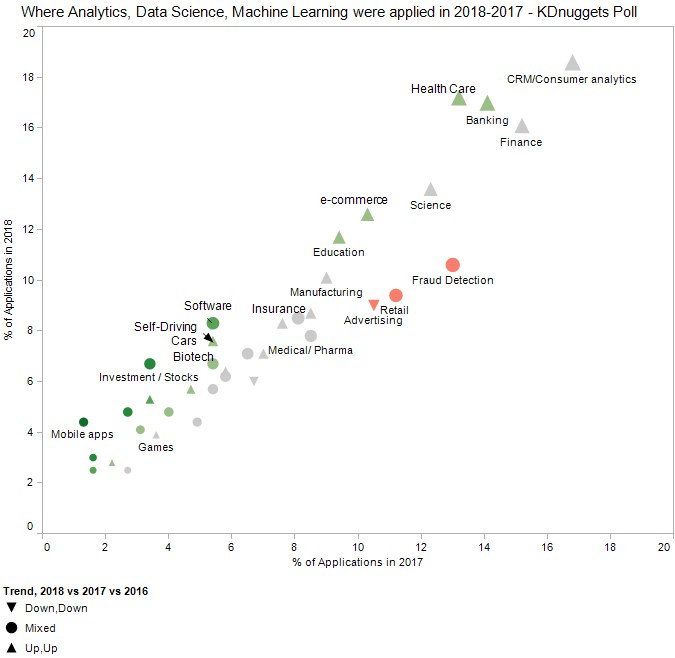
\includegraphics[width=11cm]{P1F1}
	\caption{2017年,2018年数据科学和机器学习的应用领域 —— KDnuggets 民意调查} \label{P1F1}
\end{figure}

数据科学在科学研究中非常有用。数据技术可以挖掘隐藏在海量数据中的信息和知识,为人类的社会经济活动提供基础,从而提高各个领域的运作效率,大大提高整个社会经济程度的耦合化程度。在我国,大数据将集中在以下三个领域:商业情报,政府决策和公共服务。例如:商业智能技术,政府决策技术,电信数据信息处理与挖掘技术,电网数据信息处理与挖掘技术,气象信息分析技术,环境监控技术,警务云应用系统(道路监控,视频监控,网络监控,智能交通,反电信欺诈,指挥和调度等公共安全信息系统,大规模基因序列分析和比较技术,Web信息挖掘技术,多媒体数据并行处理技术,影视制作渲染技术,云计算以及其他行业中的大量数据处理应用技术。

\subsection{数据科学的新技术}
\qquad 数据科学已成为社会变革的组成部分。 依赖数据科学,组织不再需要根据预感,猜测或小型调查做出重要决策。 取而代之的是,他们正在分析大量真实数据,基于数据驱动的真实事实做出决策。 这就是数据科学的全部意义所在——通过数据创造价值。

\textbf{1. 自动化数据分析}

即使在当今的数字时代,数据科学仍然需要大量的手动工作。 存储数据,清理数据,可视化和探索数据,最后对数据建模以获得一些实际结果。 数据科学流程的几乎每个步骤都已经或正在变得自动化。
总的来说,机构可以大量投资构建自动化数据分析的工具和服务。 这使得数据分析过程更方便。 同时,这种自动化还适合规模较小和技术含量较低的组织,这些组织可以利用这些工具和服务来访问数据科学,而无需建立专业的数据分析团队。

\textbf{2. 云上的超大型数据科学}

数据科学已经从一个小众市场发展到了应用于全方位领域的学科,可供分析的数据也呈爆炸式增长。我们手头的数据将会越来越多。

一家典型的世界500强公司可能需要分析的数据量已经远远超出了个人计算机可以处理的数据量。 一台像样的PC可能具有64GB的RAM,8核CPU和4TB的存储空间。 这对于个人项目来说效果很好,但是当他为一家拥有数百万客户数据的跨国公司(例如银行或零售商)工作时,效果就不那么理想。

\textbf{3. 自然语言处理}

在深度学习研究取得巨大突破之后,自然语言处理(NLP)开始应用于数据科学领域。深度学习在自然语言处理中取得的巨大进步推动了其与常规数据分析的全面结合。 现在,神经网络可以快速地从大量文本中提取信息。 他们能够将文本分类为不同的类别,确定关于文本的情感,并对文本数据的相似性进行分析。 最后,所有这些信息都可以存储在单个数字特征向量中。

自然语言处理成为数据科学中的强大工具。 巨大的文本数据库,使得一个单词,一个的段落,都可以转换为数值数据以进行标准分析。

\subsection{数据科学遇到的挑战}
\qquad 数据科学是一个充满潜力的领域,对从业者也有有较大需求。 但是,任何职业都会面临挑战,数据科学也不例外。 数据科学提取信息并加以利用。 但是,数据科学并非唾手可得。 在追求分析目标时,数据科学家可能会遇到各种阻碍与挑战。 在本节中,我将阐述数据科学的挑战。

在《工作中实践数据科学的十大挑战》报告中,受访者被问到,“在工作中遇到了那些阻碍与挑战?”,结果如图\ref{P1F2}所示,前十大挑战是:

\begin{enumerate}
	\item 脏数据(36\%) \\
	\item 缺乏数据科学人才(30\%) \\
	\item 公司政治(27\%) \\
	\item 缺乏明确的问题(22\%) \\
	\item 无法访问数据(22\%) \\
	\item 决策者未使用的结果(18\%) \\
	\item 向其他人解释数据科学(16\%) \\
	\item 隐私权问题(14\%) \\
	\item 缺乏领域专业知识(14\%) \\
	\item 组织规模较小,无法负担数据科学团队(13\%) \\
\end{enumerate}

\begin{figure}[h]
	\small
	\centering
	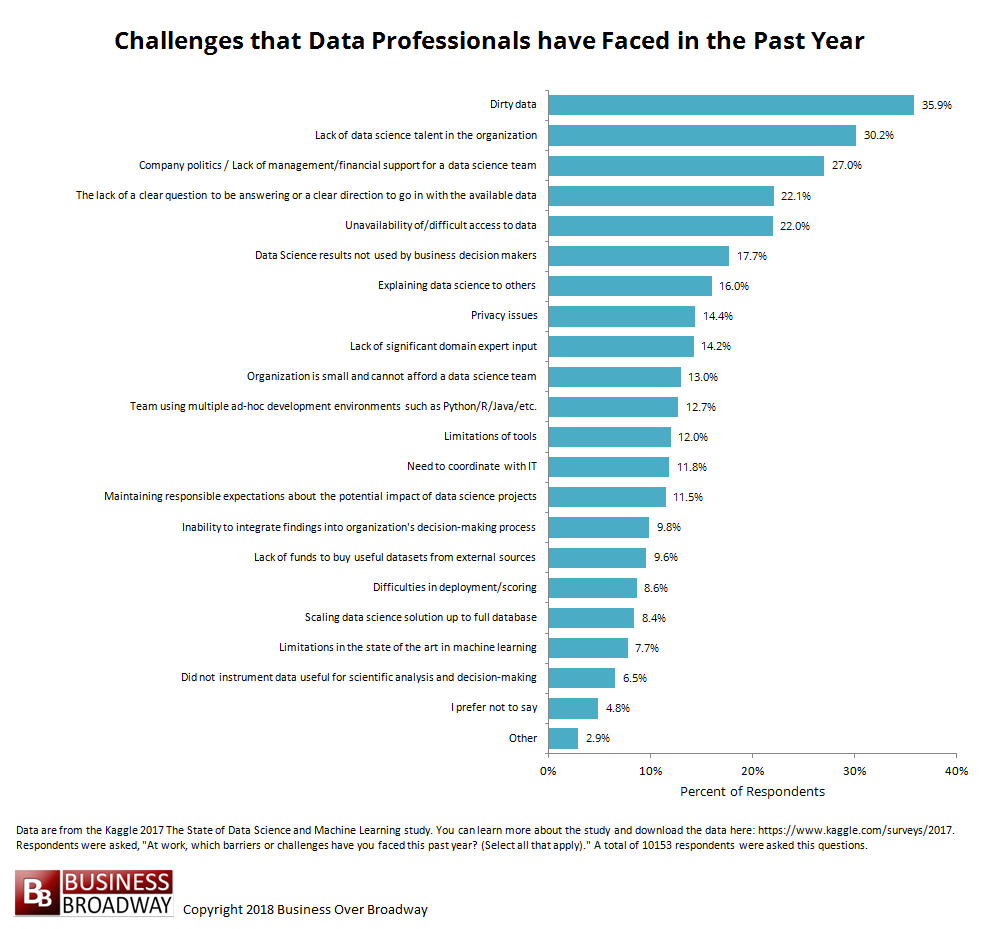
\includegraphics[width=13cm]{P1F2}
	\caption{数据科学家遇到的阻碍与挑战} \label{P1F2}
\end{figure}

结果显示,平均而言,从业者遇到了三个挑战。 经验不同的数据科学家遇到的的挑战数量差异很大。 自称是数据科学家或预测建模者的数据专业人员约有四个挑战。而自称是程序员的数据专业人员仅有一项挑战。

专业数据人员在其数据科学和机器学习中也遇到了挑战。 专业数据人员会遇到大约三个挑战。 最常见的数据科学和机器学习挑战包括脏数据,缺乏数据科学人才,缺乏管理支持以及缺乏明确的方向或问题。

\subsection{数据科学家和数据科学的前景}
\qquad 数据科学是科学过程,方法,系统和算法的交叉学科,以多种形式获取数据知识或知识。该领域结合了数据分析,统计和机器学习及其相关方法,以了解并评估数据。它使用了来自各个领域的理论和程序,数据科学家是分析数据专家,他们具有解决多方面问题的技术能力。数据科学家会处理大量结构化和非结构化的复杂数据点,并利用其能力来清理和组织它们。他们通过运用他们的分析技能来出售业务挑战,包括行业知识,上下文理解和对当前假设的怀疑。对数据科学领域感兴趣的个人通常会对数据科学家的工作前景感到疑惑。

美国劳工统计局报告,到2026年,所有计算机和信息研究科学家的就业率预计将增长19%,这被认为快于所有专业的平均水平。十年间预计将新增约5,400个工作岗位。随着数据科学领域对新技术和改进技术的需求增加,对合格数据科学家的需求也将增加。数据收集的快速增长将导致对数据挖掘服务的需求增加。

数据科学是一个不断发展的领域,在可预见的未来其需求将会增长。下面列出了一些关键变化。

1. \textbf{数据:}随着数据生成量的急剧增加,随着更多结构化数据可用于推断,预测算法的性能将随着时间的推移而提高。社交媒体和基于物联网的设备的增长加剧了这种现象,这些设备生成了更多的结构化数据。

2. \textbf{算法:}诸如遗传算法和强化学习算法之类的机器学习算法有望随着时间的推移而不断改进,从而带来更加智能的系统。

3. \textbf{分布式计算:}随着区块链技术的发展,TPU的开发以及云中可用的更快的GPU,数据科学在未来将需要功能更强大的计算硬件 。

预计在不久的将来,更多的数据以及改进的算法和硬件将共同为数据科学领域带来重大改进。

\subsection{总结}
\qquad 数据科学是一个复杂的研究领域。 在大多数情况下,数据的选择是正确的,并且可以按承诺提供解决方案。 数据科学的某些领域甚至已经开始超越人类,并且这种趋势预计在不久的将来还会增加。 我们可以参加数据科学培训以提高您的职业生涯。

数据科学是当前技术的前沿,并有望在不久的将来进一步发展技术。它也是该行业中需求最大,薪水最高的工作之一。 因此,没有比现在更好的时间成为一名数据科学家了!\\

\newpage
\begin{thebibliography}{99}
	\addcontentsline{toc}{subsection}{参考文献}
	\bibitem{1}Cao, L. (2017). Data Science: A Comprehensive Overview. ACM Computing Surveys, 50(3).
	\bibitem{2}van der Aalst W. (2016) Data Science in Action. In: Process Mining. Springer, Berlin, Heidelberg
	\bibitem{3}Banton, C. (2019). Inside Data Science and Its Applications. Retrieved 8 June 2020, from https://www.investopedia.com/terms/d/data-science.asp
	\bibitem{4}Data mining. (2020). Retrieved 8 June 2020, from https://en.wikipedia.org/wiki/Data\_mining
	\bibitem{5}Data analysis. (2020). Retrieved 8 June 2020, from https://en.wikipedia.org/wiki/D
	ata\_analysis
	\bibitem{6}Mayo, M. (2019). Where Analytics, Data Science, Machine Learning Were Applied:
	Trends and Analysis - KDnuggets. Retrieved 8 June 2020, from https://www.kdnuggets.com
	/2019/03/poll-analytics-data-science-ml-applied-2018.html
	\bibitem{7}How is the job outlook for data scientists?. (2020). Retrieved 8 June 2020, from https://www.datasciencedegreeprograms.net/faq/job-outlook-data-scientists/
	\bibitem{8}Hayes, B. (2020). Top 10 Challenges to Practicing Data Science at Work. Retrieved 8 June 2020, from https://businessoverbroadway.com/2018/03/18/top-10-challenges-to-practicing-data-science-at-work
	\bibitem{9}Seif, G. (2020). The 4 Hottest Trends in Data Science for 2020 - KDnuggets. Retrieved 8 June 2020, from https://www.kdnuggets.com/2019/12/4-hottest-trends-data-science-2020.html
\end{thebibliography}


\newpage
\subsection*{附录}
\addcontentsline{toc}{subsection}{附录}
\subsubsection*{附录 A: 数据科学的应用领域统计}
% Please add the following required packages to your document preamble:
% \usepackage[table,xcdraw]{xcolor}
% If you use beamer only pass "xcolor=table" option, i.e. \documentclass[xcolor=table]{beamer}
\begin{table}[H]
	\begin{tabular}{
			>{\columncolor[HTML]{FFFFFF}}l 
			>{\columncolor[HTML]{FFFFFF}}l 
			>{\columncolor[HTML]{FFFFFF}}l 
			>{\columncolor[HTML]{FFFFFF}}l }
		\hline
		{\color[HTML]{1F0909} \textbf{领域}}      & {\color[HTML]{1F0909} \textbf{2018}} & {\color[HTML]{1F0909} \textbf{2017}} & {\color[HTML]{1F0909} \textbf{2016}} \\ \hline
		{\color[HTML]{1F0909} CRM /消费者分析(81)}   & {\color[HTML]{1F0909} 18.60}         & {\color[HTML]{1F0909} 16.80}         & {\color[HTML]{1F0909} 16.30}         \\
		{\color[HTML]{1F0909} 卫生保健(75)}         & {\color[HTML]{1F0909} 17.20}         & {\color[HTML]{1F0909} 13.20}         & {\color[HTML]{1F0909} 12.00}         \\
		{\color[HTML]{1F0909} 银行(74)}           & {\color[HTML]{1F0909} 17.00}         & {\color[HTML]{1F0909} 14.10}         & {\color[HTML]{1F0909} 13.40}         \\
		{\color[HTML]{1F0909} 金融(70)}           & {\color[HTML]{1F0909} 16.10}         & {\color[HTML]{1F0909} 15.20}         & {\color[HTML]{1F0909} 15.00}         \\
		{\color[HTML]{1F0909} 科学(59)}           & {\color[HTML]{1F0909} 13.60}         & {\color[HTML]{1F0909} 12.30}         & {\color[HTML]{1F0909} 12.00}         \\
		{\color[HTML]{1F0909} 电子商务(55)}         & {\color[HTML]{1F0909} 12.60}         & {\color[HTML]{1F0909} 10.30}         & {\color[HTML]{1F0909} 8.90}          \\
		{\color[HTML]{1F0909} 教育(51)}           & {\color[HTML]{1F0909} 11.70}         & {\color[HTML]{1F0909} 9.40}          & {\color[HTML]{1F0909} 7.10}          \\
		{\color[HTML]{1F0909} 欺诈检测(46)}         & {\color[HTML]{1F0909} 10.60}         & {\color[HTML]{1F0909} 13.00}         & {\color[HTML]{1F0909} 11.10}         \\
		{\color[HTML]{1F0909} 制造业(44)}          & {\color[HTML]{1F0909} 10.10}         & {\color[HTML]{1F0909} 9.00}          & {\color[HTML]{1F0909} 5.60}          \\
		{\color[HTML]{1F0909} 零售(41)}           & {\color[HTML]{1F0909} 9.40}          & {\color[HTML]{1F0909} 11.20}         & {\color[HTML]{1F0909} 10.30}         \\
		{\color[HTML]{1F0909} 广告(39)}           & {\color[HTML]{1F0909} 9.00}          & {\color[HTML]{1F0909} 10.50}         & {\color[HTML]{1F0909} 12.00}         \\
		{\color[HTML]{1F0909} 供应链(38)}          & {\color[HTML]{1F0909} 8.70}          & {\color[HTML]{1F0909} 8.50}          & {\color[HTML]{1F0909} 6.50}          \\
		{\color[HTML]{1F0909} 保险(37)}           & {\color[HTML]{1F0909} 8.50}          & {\color[HTML]{1F0909} 8.10}          & {\color[HTML]{1F0909} 9.20}          \\
		{\color[HTML]{1F0909} 软件(36)}           & {\color[HTML]{1F0909} 8.30}          & {\color[HTML]{1F0909} 5.40}          & {\color[HTML]{1F0909} 7.20}          \\
		{\color[HTML]{1F0909} IT /网络基础设施(36)}   & {\color[HTML]{1F0909} 8.30}          & {\color[HTML]{1F0909} 7.60}          & {\color[HTML]{1F0909} 7.20}          \\
		{\color[HTML]{1F0909} 其他(34)}           & {\color[HTML]{1F0909} 7.80}          & {\color[HTML]{1F0909} 8.10}          & {\color[HTML]{1F0909} 6.30}          \\
		{\color[HTML]{1F0909} 医疗/制药(34)}        & {\color[HTML]{1F0909} 7.80}          & {\color[HTML]{1F0909} 8.50}          & {\color[HTML]{1F0909} 6.50}          \\
		{\color[HTML]{1F0909} 汽车/自动驾驶汽车(33)}    & {\color[HTML]{1F0909} 7.60}          & {\color[HTML]{1F0909} 5.40}          & {\color[HTML]{1F0909} 4.50}          \\
		{\color[HTML]{1F0909} 石油/天然气/能源(31)}    & {\color[HTML]{1F0909} 7.10}          & {\color[HTML]{1F0909} 6.50}          & {\color[HTML]{1F0909} 7.10}          \\
		{\color[HTML]{1F0909} 信用评分(31)}         & {\color[HTML]{1F0909} 7.10}          & {\color[HTML]{1F0909} 7.00}          & {\color[HTML]{1F0909} 6.90}          \\
		{\color[HTML]{1F0909} 投资/股票(29)}        & {\color[HTML]{1F0909} 6.70}          & {\color[HTML]{1F0909} 3.40}          & {\color[HTML]{1F0909} 6.20}          \\
		{\color[HTML]{1F0909} 生物技术/基因组学(29)}    & {\color[HTML]{1F0909} 6.70}          & {\color[HTML]{1F0909} 5.40}          & {\color[HTML]{1F0909} 5.80}          \\
		{\color[HTML]{1F0909} 政府/军事(28)}        & {\color[HTML]{1F0909} 6.40}          & {\color[HTML]{1F0909} 5.80}          & {\color[HTML]{1F0909} 5.60}          \\
		{\color[HTML]{1F0909} 电信/电缆(27)}        & {\color[HTML]{1F0909} 6.20}          & {\color[HTML]{1F0909} 5.80}          & {\color[HTML]{1F0909} 8.30}          \\
		{\color[HTML]{1F0909} 社交媒体/社交网络(26)}    & {\color[HTML]{1F0909} 6.00}          & {\color[HTML]{1F0909} 6.70}          & {\color[HTML]{1F0909} 8.30}          \\
		{\color[HTML]{1F0909} 人力资源/劳动力分析(25)}   & {\color[HTML]{1F0909} 5.70}          & {\color[HTML]{1F0909} 4.70}          & {\color[HTML]{1F0909} 3.60}          \\
		{\color[HTML]{1F0909} 搜索/ Web内容挖掘(25)}  & {\color[HTML]{1F0909} 5.70}          & {\color[HTML]{1F0909} 5.40}          & {\color[HTML]{1F0909} 5.40}          \\
		{\color[HTML]{1F0909} 农业(23)}           & {\color[HTML]{1F0909} 5.30}          & {\color[HTML]{1F0909} 3.40}          & {\color[HTML]{1F0909} 3.30}          \\
		{\color[HTML]{1F0909} 娱乐/音乐/电视/电影(21)}  & {\color[HTML]{1F0909} 4.80}          & {\color[HTML]{1F0909} 2.70}          & {\color[HTML]{1F0909} 4.00}          \\
		{\color[HTML]{1F0909} 旅行/款待(21)}        & {\color[HTML]{1F0909} 4.80}          & {\color[HTML]{1F0909} 4.00}          & {\color[HTML]{1F0909} 4.00}          \\
		{\color[HTML]{1F0909} 行动应用程式(19)}       & {\color[HTML]{1F0909} 4.40}          & {\color[HTML]{1F0909} 1.30}          & {\color[HTML]{1F0909} 3.30}          \\
		{\color[HTML]{1F0909} 直接营销/筹款(19)}      & {\color[HTML]{1F0909} 4.40}          & {\color[HTML]{1F0909} 4.90}          & {\color[HTML]{1F0909} 4.30}          \\
		{\color[HTML]{1F0909} 采矿(18)}           & {\color[HTML]{1F0909} 4.10}          & {\color[HTML]{1F0909} 3.10}          & {\color[HTML]{1F0909} 4.20}          \\
		{\color[HTML]{1F0909} 游戏(17)}           & {\color[HTML]{1F0909} 3.90}          & {\color[HTML]{1F0909} 3.60}          & {\color[HTML]{1F0909} 2.90}          \\
		{\color[HTML]{1F0909} 安全/反恐(13)}        & {\color[HTML]{1F0909} 3.00}          & {\color[HTML]{1F0909} 1.60}          & {\color[HTML]{1F0909} 2.70}          \\
		{\color[HTML]{1F0909} 垃圾电子邮件/反垃圾邮件(12)} & {\color[HTML]{1F0909} 2.80}          & {\color[HTML]{1F0909} 2.20}          & {\color[HTML]{1F0909} 1.10}          \\
		{\color[HTML]{1F0909} 社会政策/调查分析(11)}    & {\color[HTML]{1F0909} 2.50}          & {\color[HTML]{1F0909} 1.60}          & {\color[HTML]{1F0909} 1.80}          \\
		{\color[HTML]{1F0909} 社会公益/非营利组织(11)}   & {\color[HTML]{1F0909} 2.50}          & {\color[HTML]{1F0909} 2.70}          & {\color[HTML]{1F0909} 2.00}          \\ \hline
	\end{tabular}
\end{table}

\newpage
\subsubsection*{附录 B: 40种数据科学常用技术}
\begin{table}[H]
	\begin{tabular}{ll}
		线性回归          & (地理)空间建模 \\
		逻辑回归          & 推荐引擎     \\
		折刀回归          & 搜索引擎     \\
		密度估算          & 归因建模     \\
		置信区间          & 协同过滤     \\
		假设检验          & 规则系统     \\
		模式识别          & 连锁分析     \\
		聚类-(又名无监督学习)  & 关联规则     \\
		监督学习          & 计分引擎     \\
		时间序列          & 分割       \\
		决策树           & 预测建模     \\
		随机数           & 图表       \\
		蒙特卡洛模拟        & 深度学习     \\
		贝叶斯统计         & 博弈论      \\
		朴素贝叶斯         & 归因       \\
		主成分分析-(PCA)   & 生存分析     \\
		合奏            & 套利       \\
		神经网络          & 举升模型     \\
		支持向量机-(SVM)   & 产量优化     \\
		最近的邻居-(k-NN)  & 交叉验证     \\
		特征选择-(又称可变约简) & 模型拟合     \\
		索引/编目         & 相关性算法   
	\end{tabular}
\end{table}

\newpage
\section{公开数据集的介绍与我对数据公开的看法}
\subsection{政府数据集介绍}
\qquad 在本节中,我将介绍新西兰政府的两个数据集。

本部分中的所有数据均来自新西兰政府数据公开平台(data.govt.nz),并遵循CC 4.0 BY-SA版权协议
\subsubsection{第一个数据集介绍:PM2.5浓度,2008-17}
\qquad PM2.5由空气中直径小于2.5微米的固体和液体颗粒组成。 在新西兰,空气中的大多数PM2.5来自燃烧(燃烧木材以供家庭取暖,机动车排气),并且在较小程度上是由大气中的反应和天然存在的海盐形成的颗粒。 短期和长期暴露于PM2.5(即使是低水平)也与呼吸道和心血管疾病以及过早死亡的风险增加有关,尤其是在弱势人群(年轻人,老年人和患有呼吸道疾病的人群)中。 该数据集记录了2008年至2017年每天PM2.5的浓度。

该数据集包含要测试的城市的数据,测试的日期,测试机构,测试方法,PM2.5值以及是否完整记录了当年的所有数据。记录创建于2020年2月2日,最后更新时间为2020年6月2日。

我将数据集导入到R中,并试图查看数据集的结构。 幸运的是,该数据集的数据几乎不需要清理,数据非常干净。 我们可以通过ggplot轻松查看数据的结构和特征。这份数据有很多非常有趣的特征,这些特征让我非常惊讶,结果也很有趣。

\textbf{1. 首先将数据集导入R中}
\begin{minted}%
[encoding=utf8,
linenos,
frame=single,
rulecolor=purple!50!black,
texcl=true,
highlightcolor=green!40,
]{R}
library(tidyverse)
library(lubridate)
setwd("C:/Users/tclkr/Desktop/D1")
pm25<-read_csv("./pm25.csv")
\end{minted}

\textbf{2.起初,我只想对PM2.5的每日数据进行汇总并绘图,从而查看PM2.5浓度的变化规律}
\begin{minted}%
[encoding=utf8,
linenos,
frame=single,
rulecolor=purple!50!black,
texcl=true,
highlightcolor=green!40,
]{R}
byy<-pm25%>%
  select(site,date,pm2_5)%>%
  group_by(date)%>%
  summarize(val=mean(pm2_5,na.rm=TRUE))

ggplot(data=byy)+
  geom_point(mapping = aes(x=date,y=val),size=0.35)+
  labs(x="日期",y="浓度")
\end{minted}
\begin{figure}[h]
	\small
	\centering
	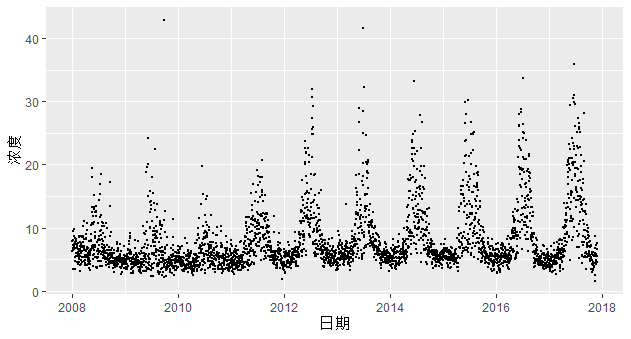
\includegraphics[width=13cm]{P2F1}
	\caption{PM2.5历史每日浓度变化图} \label{P2F1}
\end{figure}

在图\ref{P2F1}中, PM2.5浓度总体呈现上升趋势,但是每年都会先上升后下降,这引起了我的研究兴趣。

\textbf{3. 我想计算每个月PM2.5的平均浓度}
\begin{minted}%
[encoding=utf8,
linenos,
frame=single,
rulecolor=purple!50!black,
texcl=true,
highlightcolor=green!40,
breaklines=true,
]{R}
bymon_day<-pm25%>%
  select(date,pm2_5)%>%
  mutate(date_in_year=make_date(2020,month(date),day(date)))%>%
  group_by(date_in_year)%>%
  summarize(mean_value=mean(pm2_5,na.rm=TRUE))

ggplot(data=bymon_day,mapping = aes(x=date_in_year,y=mean_value))+
  geom_point(alpha=0.3)+
  geom_smooth(method="loess")+
  scale_x_date(date_breaks = "1 month", date_minor_breaks = "1 month", date_labels = "%b")+
  labs(x="日期",y="浓度")
\end{minted}
\begin{figure}[h]
	\small
	\centering
	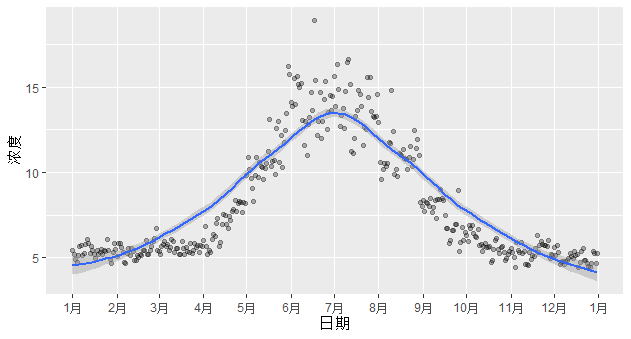
\includegraphics[width=13cm]{P2F2}
	\caption{月均PM2.5浓度变化图} \label{P2F2}
\end{figure}

如我所想, 在图\ref{P2F2}中PM2.5浓度在一年中先上升后下降,但是我没有想到回归曲线是如此规则,置信区间很小,这使我想通过QQ图(图\ref{P2F3})来研究其正态分布相关性

\begin{minted}%
[encoding=utf8,
linenos,
frame=single,
rulecolor=purple!50!black,
texcl=true,
highlightcolor=green!40,
]{R}
ggplot()+
  qqnorm(bymon_day$mean_value)
\end{minted}
\begin{figure}[h]
	\small
	\centering
	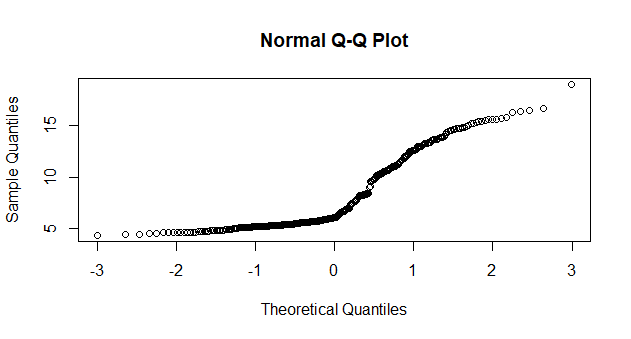
\includegraphics[width=13cm]{P2F3}
	\caption{PM2.5浓度月平均变化图的QQ图} \label{P2F3}
\end{figure}

\textbf{4.然后我查看了每年之间的PM2.5浓度变化(图. \ref{P2F4})}

\begin{minted}%
[encoding=utf8,
linenos,
frame=single,
rulecolor=purple!50!black,
texcl=true,
highlightcolor=green!40,
]{R}
byyear<-pm25%>%
  select(site,date,pm2_5)%>%
  mutate(years=year(date))%>%
  group_by(years)%>%
  summarize(val=mean(pm2_5),na.rm=TRUE)

ggplot(data=byyear,aes(x=years,y=val))+
  geom_line()+
  geom_point()+
  labs(x="日期",y="浓度")
\end{minted}
\begin{figure}[h]
	\small
	\centering
	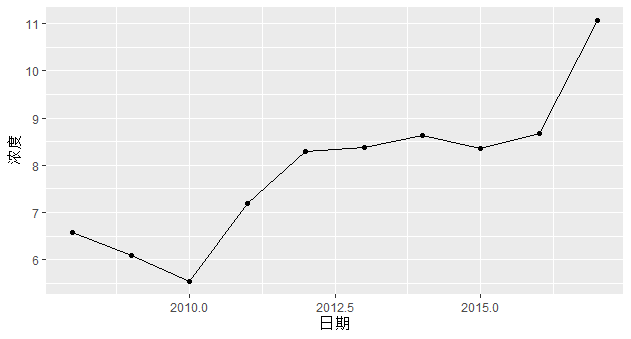
\includegraphics[width=12cm]{P2F4}
	\caption{PM2.5浓度年变化图} \label{P2F4}
\end{figure}

遗憾的是我无法解释为什么PM2.5的浓度在2008年至2010年之间急剧下降

\textbf{5. 最后,我查看了每个城市的平均数据}

\begin{minted}%
[encoding=utf8,
linenos,
frame=single,
rulecolor=purple!50!black,
texcl=true,
highlightcolor=green!40,
]{R}
bycty<-pm25%>%
  select(site,date,pm2_5)%>%
  group_by(site)%>%
  summarize(val=mean(pm2_5),na.rm=TRUE)
library(maps)
library(mapdata)
library(maptools)
library(rgdal)
map<-readOGR("./NZL_adm2.shp")
map1 <- fortify(map)
map1 <- as_tibble(map1)
map1 <- filter(map1,long>50)
ggplot()+
  geom_map(mapping = aes(x=map1$long,y=map1$lat))
\end{minted}

\subsubsection{第二个数据集介绍:癌症历史摘要1948-2011}
\qquad 该数据集为1948年至2011年癌症部位记录和死亡数据汇总。该数据创建于2018年5月21日。部位包括:嘴唇,嘴巴和咽,食道,胃,大肠,肝脏和肝内胆管, 胰腺,肺,黑色素瘤,乳腺癌,子宫颈,子宫,卵巢,外阴,肾脏,膀胱,脑,甲状腺,霍奇金淋巴瘤,非霍奇金淋巴瘤,骨髓瘤,白血病。 记录死亡人数和ASR值

可以用很多方法来找出它们之间的关系。 例如,可以找到时间和癌症类型之间的关系,癌症类型的比例的关系,等等。

\subsection{数据公开的优点}
\qquad 开放数据是一种重要信息,可不受限制免费提供给任何人。 各国政府都十分看重这种与居民联系的新方法,这一行动已被称为政府数据公开。 许多政府机构已经开始认识到开放和透明数据行动的好处。 从立法,政策和实践到政府绩效的信息都可以向公众公开。

\textbf{1. 提高透明度并强化问责制}

开放数据的趋势意味着公众可以与政府保持联系,了解最新信息并保持最新状态。 这些信息的公共性质要求政府对其产生的结果负责。 居民有能力准确了解其政府取得的成果以及需要做的工作。 未能达到某些结果或未达到特定目标的情况将公布,并接受公众问责。 相反,如果政府达到或超越目标将有助于与当地居民建立更号的信任关系。

\textbf{2. 建立信任,信誉和声誉}

可公开访问的数据全方位的描述了组织的另一面,黑幕将无法被保存。 这种开放性和脆弱性相当于与他人分享您个人生活的各个方面。 公开而真诚的交互伴随着相当多的信任和尊重,结果往往是两方之间的关系更加紧密和相互依赖。 同样,公开的政府数据有助于建立与公民的信任和信誉。 开放数据可使居民放心,他们的地方政府可以不断努力兑现承诺并为社区的最大利益做出决策。

\textbf{3. 促进进步与创新}

关键绩效数据的价值在公共领域宽松时几乎没有限制。 开放数据为商业应用提供了新的机会,缩短了产品的上市时间,并可以为新技术创新和经济增长奠定基础。 不需要依赖于收集这些数据的第三方机构,所有人可以利用该信息开发新的应用程序和服务。 以这种方式提供的信息对于学术界,公共部门和基于行业的研究社区也很重要。 开放数据极大地增加了信息的价值,并使信息得以传播并被充分利用。

\textbf{4. 促进公众教育与社区参与}

有什么比将所有信息显示在清晰,人性化的显示屏上更好的方式来教育社区有关城市的进步和表现的方法? 开放的政府数据使您可以通过自由访问信息来主动回答那些常见问题。 信息可以在收集后尽快提供,这意味着公众可以参与其中并在整个过程中提供有价值的反馈。 访问有意义的数据有助于统一社区并赋予他们权力以帮助塑造未来的方向。

\textbf{5. 提高公民参与度}

公民期望参与民主的活动,但由于缺乏信息获取,他们几乎无法参与。 开放数据可以促进公民参与。

\subsection{数据公开的缺点}
\qquad \textbf{1. 开放数据存在违反法规的风险}

由于法律或其他原因,许多数据集已经或不能发布。 不能向公众提供的数据集示例包括包含隐私标识变量,敏感变量的数据集,以及由具有不同安全级别,不同政策并必须遵守不同法律的多个组织创建的数据集。 发布此类数据将导致不良情况,因为这将违反法律并可能损害提供这些数据的组织的声誉。

\textbf{2. 数据版权问题}

在一次采访中,有人说政府组织还维护其他组织的数据。 这些数据不属于政府组织所有,因此无法发布。 此外,当其他组织为数据的创建做出了贡献时,这些数据将无法发布。 “借来的数据”的影响很大。 许多研究都是基于借来的数据。 这主要涉及从其他政府组织借来的数据。 提到不与其他组织一起发布借用或创建的数据的主要原因是,该组织不想冒名誉受损的风险,正如一位员工所说的那样:“一个人想打开数据,但不放心所有东西”。

\textbf{3. 隐私可能会被无意侵犯}

在从数据集中删除隐私敏感变量方面已付出了很多努力,以便可以打开它们。 有人可能会认为隐私得到了保障。 尽管如此,通过将数据与其他来源合并起来,仍然有可能跟踪一个人的身份,尤其是当开放数据与社交媒体数据结合在一起时。 有关隐私敏感性的准则部分有助于确定哪些数据无法发布,但仍需要数据提供者做出大量解释,并且合并数据仍可能导致识别个人身份。

\textbf{4. 存在误解和滥用}

公众无法获得非常复杂的数据,因为这些数据集被误解和滥用的风险很高。 此外,在其中一个组织中,发现一些数据集的文档记录太差,无法正确解释数据。 作为开放数据提供的数据可免费提供给任何人。 这也意味着对如何解释开放数据了解有限的人可以使用它们。 这可能会导致有关数据分析结果的错误结论。 有些人甚至可能打算滥用数据以破坏数据提供者的声誉。

\subsection{对我国政府数据公开的建议}
\qquad \textbf{1. 政府应改善平台服务}

在学习数据科学导论时,我尝试从许多中国政府数据开放平台下载数据,但是许多平台的许多数据请求功能未能及时有效地响应。 有很多的平台,其反馈没有及时得到答复,而该平台的维护者应对于用户的问题和存在的问题作出回应,关注用户反馈和需求的过程中,解决了用户的问题。 用户的数据需求应及时得到回应,如果无法提供数据,则还必须说明保密的原因。

\textbf{2. 开放平台应加强与用户的互动}

注册后,我们的政府数据开放平台应该提供交流功能。 一些平台注册需要使用身份证实名认证,这增加了用户与平台之间进行交流的门槛,并降低了消息交互的自由度。

\textbf{3. 政府应鼓励数据开发和利用}

目前,数千种应用程序和软件工具以及数百种手机软件被应用到美国政府数据开放平台(data.gov)。这些应用程序中有超过三分之一是由私人程序员和非营利组织开发的。尽管中国政府数据开放平台还启动了创新的APP活动,但公众的参与度很低,这无法调动参与的兴趣。我国政府有许多数据开放平台无法满足公众参与创新APP的数据需求。在某些平台上,交流仅限于经过批准的企业用户,其受众相对狭窄,极大地损害了用户的热情和创造力。因此,中国政府数据开放平台应首先提高平台自身的数据质量,然后进行更多的互动,可以适当地提供一些奖励,以激发人们对参与的兴趣。

\newpage
\begin{thebibliography}{99}
	\addcontentsline{toc}{subsection}{参考文献}
	\bibitem{1}Cancer: Historical summary 1948-2011 - data.govt.nz - discover and use data. (2018). Retrieved 31 December 1921, from https://catalogue.data.govt.nz/dataset/cancer-historical-summary-1948-2011
	\bibitem{1}PM2.5 concentrations, 2008–17 - data.govt.nz - discover and use data. (2020). Retrieved 9 June 2020, from https://catalogue.data.govt.nz/dataset/pm2-5-concentrations-200817
	\bibitem{3}Zhang, J. (2018). Research on the development status and countermeasures of Chinese government data opening platform. Heilongjiang: Heilongjiang University.
	\bibitem{4}Wang, L. (2017). Research on government Data Opening from the perspective of holistic governance. Wuhan: Central China Normal University.
	\bibitem{5}Starting an Open Data Initiative. (2019). Retrieved 9 June 2020, from http://opendatatoolkit.worldbank.org/en/starting.html
	\bibitem{6}6 Major Benefits of Open Data – ProWebScraper. Retrieved 9 June 2020, from https://prowebscraper.com/blog/6-major-benefits-of-open-data/
	\bibitem{7}Ong, C. (2016). 5 Benefits of Open Government Data | Envisio. Retrieved 9 June 2020, from https://envisio.com/blog/5-benefits-of-open-government-data/
	\bibitem{8}Pros and Cons of Open Data. (2018). Retrieved 9 June 2020, from https://thesciencefactor.wordpress.com/2018/03/31/pros-and-cons-of-open-data-wcri2017/
	\bibitem{9}Zuiderwijk, A., \& Janssen, M. (2014). The negative effects of open government data - investigating the dark side of open data. digital government research.
\end{thebibliography}

\newpage

\section{流行病定量分级与COVID-19无症状感染者预测模型}
\subsection*{摘要}
\addcontentsline{toc}{subsection}{摘要}
\textbf{人类的伟大是勇气的伟大,人类的赞歌是勇气的赞歌。}
\begin{flushright}\textbf{—— JoJo的奇妙冒险}\end{flushright}
\vspace{0.7cm}

\textit{截止摘要撰写时(2020年6月11日),COVID-19已经造成了7221717例感染,其中411818例死亡。中国在抗击肺炎疫情时做出来巨大的牺牲,同时其积极的策略使得肺炎传播得到了快速控制,中国的行为获得了WHO高度赞赏。此时,我们已经实现了大部分行业的复工复产。其他国家的情况则不容乐观,例如美国疫情的发展状态令人十分费解,在央视新闻发出的"中国以外新冠肺炎累计确诊20000例以上的国家"统计柱状图中,美国的人数实在是太多了以至于柱状图不得不拐两个弯才画的完,让国内外网友戏称出现拐点。美国政府的言论同样让人费解,政府告诉人们不要戴口罩,通过喝消毒水预防新冠肺炎。最令人惊讶的是美国在与WHO多次相互批评后竟退出了WHO。美国政府曾认为WHO提出COVID-19疫情进入到了全球大流行阶段对造成不必要的恐慌,理由是SARS 尽管影响了26 个国家,但仍未被认为是大流行病,MERS也没有被认为是大流行病。引起这一争论的原因是WHO对于疾病是否达到全球大流行没有定量的严格标准,也没有定义的病例或死亡数量阈值。}

\textit{无症状感染者的存在是另一个让疫情防控充满困难的因素,无症状感染者具有一定的传染性,且不容易发现。在中国复工复产的过程中,很多地区出现了核酸检测阳性的无症状感染者,“无症状感染者”似乎成为了新的传染源。在网络中,我们可以找到很多对于COVID-19疫情发展的预测,但是很难得到无症状感染者人数的预测数据。}

\textit{基于以上两点,我通过新冠肺炎在各国的传播数据并结合H1N1, SARS, MERS的传播数据得到疾病大流行的定量标准,并获得无症状感染者感染人数的预测模型}

\textit{对于何为疾病全球大流行的问题中,我选取了 16 种较为著名的流行病,并考虑了11种评价指标。首先,我选用了 R 型聚类法对指标进行降维处理;接着,借助流行病学对传染病的分类,选用了 Q 型聚类法将 11种疾病分成了四大类:散发,暴发、流行和大流行,实现各级别之间的定量化识别。最后,我根据主成分分析法对不同类别传染病进行综合评价,合理量化了“流行”和“大流行”病的界限。}

\textit{针对无症状感染者人数预测,我以重庆市与湖北省为例,分别从统计学和病毒传播动力学病学两个方面展开分析。在病毒传播动力学角度我采用针对COVID-19改进的SEIR方法进行预测,在统计学方面,我选用了响应面预测模型对改进的SEIR模型进行正确性验证。}
\\
\textbf{关键词:}\textit{聚类分析;主成分分析;修正 SEIR 模型;COVID-19;响应面预测模型}\\

\newpage
\subsection{问题假设}
\qquad 在数据分析与预测之前我们给出以下假设:

1. 短期内无特效药出现。

2. 政府采取的疫情防控严格程度不变。

3. 不会出现海外华人大量回国与国内特大规模的人员聚集与流动

\subsection{数据集的介绍}
\qquad 我们可以在WHO与各国卫生部门获得该国的疫情传播数据,我在GitHub上找到了一个较为优秀的数据集"datasets/covid-19", 这个数据集由约翰霍普金斯大学系统科学和工程中心的“amazing”团队维护。该团队每天都将世界卫生组织, 中国丁香园,BNO新闻,中国国家卫生委员会(NHC), 中国疾控中心(CCDC), 香港卫生署, 澳门政府, 台湾疾控中心, 美国疾控中心, 加拿大政府, 澳大利亚政府卫生部, 欧洲疾控中心, 新加坡卫生部, 意大利卫生部 公布的数据汇总到该数据集中。由于目前全球大部分国家疫情逐步被控制,此时数据多样性较低,我们选取了2020年4月19日(即湖北省首次患者清零后一月)的镜像数据进行分析,此时在不同的国家病毒发展状况不尽相同。

数据集包含7个CSV文件,包含每日按国家拼写排序的感染死亡人数,每日主要感染国家感染数,各国各州/省份经纬度与人口数,以州/省聚合的地理位置与感染人数,美国各乡镇感染人数与地理位置,美国各乡镇死亡人数与地理位置,世界感染死亡总数据,其中“每日按国家拼写排序的感染死亡人数”,“每日主要感染国家感染数"可以由"以州/省聚合的地理位置与感染人数"表示,故我们不使用以上两文件,”各国各州/省份经纬度与人口数“可以被连接到”以州/省聚合的地理位置与感染人数“。最后我们得到三个数据集:美国各州,全球各国家(省份),全球汇总表。

\subsection{数据预处理}
\qquad 1. \textbf{数据的合并与转换:}我们先将上述文件读入(附录C 1-16行),合并数据,生成三个全新的数据集(附录C 17-78行)。

2. \textbf{冗余数据的处理:}数据集中有部分冗余数据列如iso2、iso3、code3列,这些列数据为GIS软件中对于国家与地区的编码,在本次数据分析中没有作用,故剔除之(附录C 42,43行)。

3. \textbf{异常值处理:}在异常数据处理之前,我们先绘制了全球当日存在的患者数目(附录C 80-85行),发现其仍处于增加状态(图 \ref{P3F1}),故无法通过常规的$3\sigma$法则对于进行异常值剔除,故没有做异常值剔除工作

\begin{figure}[h]
	\small
	\centering
	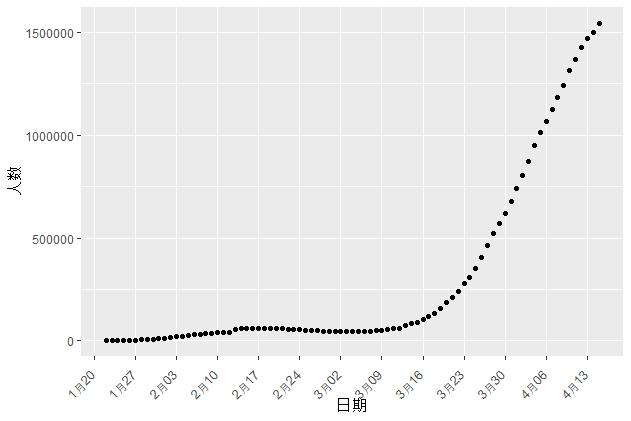
\includegraphics[width=13cm]{P3F1}
	\caption{感染人数随时间变化} \label{P3F1}
\end{figure}

4. \textbf{数据完整性分析:}通过计算数据集中有效值占比获得数据的完整度(附录C 87-93行),部分结果如表\ref{P3T1} 所示(在代码中给出了两种合并方式,方案一需要使用自己写的主键生成函数,但是对主键进行了数据预处理,使得人口经纬度数据完整度达到98.11\%与98.86\%。方案二使用双键作为主键,但是人口与经纬度数据完整度为68\%) 
% Please add the following required packages to your document preamble:
% \usepackage[table,xcdraw]{xcolor}
% If you use beamer only pass "xcolor=table" option, i.e. \documentclass[xcolor=table]{beamer}
\begin{table}[H]
	\caption{数据完整度} \label{P3T1}
	\begin{tabular}{lllllllll}
		\hline
		\textbf{指标} & \textbf{感染人数} & \textbf{病死人数} & \textbf{治愈人数} & \textbf{时间} & \textbf{国家} & \textbf{增长率} & \textbf{人口数} & \textbf{经纬度} \\ \hline
		完整度         & 99.62\%       & 99.62\%       & 94.69\%       & 100\%         & 100\%         & 99.62\%      & 98.11\%      & 98.86\%      \\ \hline
	\end{tabular}
\end{table}

5. \textbf{变量相关性分析:}对于变量相关性分析一般考虑如下方法:1. 欧几里得算法2. 皮尔逊相关系数算法3. 夹角余弦公式,其中欧几里得算法适用于数据属性较多的数据集,而余弦公式适合数据较为稀疏的数据,而皮尔逊相关系数算法适用于数据受级别膨胀影响的情况,对数据集进行summary操作可以看到皮尔逊相关系数算法比较适合本数据集的相关性分析(些变量数据之间存在数量级的差异),皮尔逊相关系数即两个变量之间的协方差和标准差的商,其表达形式为:变量$P_i$, $P_j$之间的相关系数

$$
\begin{aligned}
R_{i,j} & =\frac{P_i-\overline P_i,P_j-\overline P_j}{\|P_i-\overline P_i\|\|P_j-\overline P_j\|}
 = \frac{\sum_{m=1}^{n}(P_{im}-\overline P_i)(P_{jm}-\overline P_j)}{\left[ \sum_{m=1}^{n}(P_{im}-\overline P_i)^2 \sum_{m=1}^{n}(P_{jm}-\overline P_j)^2 \right]^{\frac{1}{2}}}\\
& =\frac{E\left[(P_i-\mu P_i)(P_j-\mu P_j)\right]}{\sigma_{P_i}\sigma_{P_j}}
 =\frac{cov(P_i,P_j)}{\sigma_{P_i}\sigma_{P_j}}  ,-1\leq R_{i,j}\leq 1
\end{aligned}
$$

对部分变量计算皮尔逊相关系数(附录C 95-107行)得到如表\ref{P3T2}与图\ref{P3F2}(附录C 109-185行):

\begin{table}[H]
	\centering
	\caption{皮尔逊相关系数} \label{P3T2}
	\begin{tabular}{|l|l|l|l|l|l|}
		\hline
		\textbf{指标}  & \textbf{日期} & \textbf{感染数} & \textbf{治愈数} & \textbf{死亡数} & \textbf{增长率} \\ \hline
		\textbf{日期}  & 1           & 0.806501     & 0.840417     & 0.765599     & -0.4506      \\ \hline
		\textbf{感染数} & 0.806501    & 1            & 0.806501     & 0.995398     & -0.21135     \\ \hline
		\textbf{治愈数} & 0.840417    & 0.98934      & 1            & 0.988752     & -0.24571     \\ \hline
		\textbf{死亡数} & 0.765599    & 0.995398     & 0.988752     & 1            & -0.19537     \\ \hline
		\textbf{增长率} & -0.4506     & -0.21135     & -0.24571     & -0.19537     & 1            \\ \hline
	\end{tabular}
\end{table}

\begin{figure}[h]
	\small
	\centering
	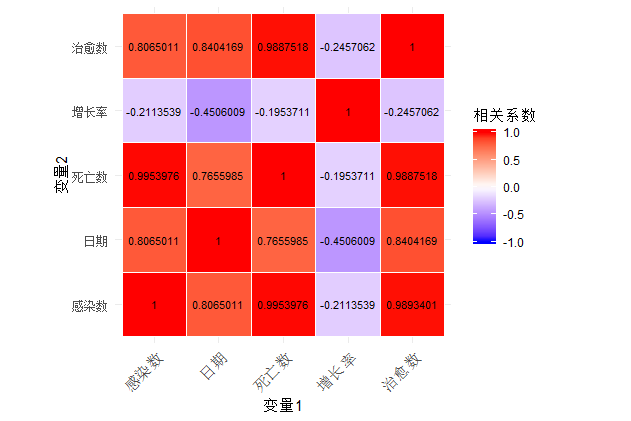
\includegraphics[width=14cm]{P3F2}
	\caption{相关系数热图} \label{P3F2}
\end{figure}

根据得到的相关系数热图,可以看出,感染人数越多,病死人数越多,对应的时间越长;感染人数越多,对应的增长率越高 但是增长率与其余变量关系不大,仅与疫情持续时间有较弱的关系。这些结论基本符合常识,也说明了传染病传播能力强弱与多个因素有关,在进行影响因素分析时,应考虑多个因素的影响

6.\textbf{数据归一化:}由于指标之间存在不同的量纲,数据大小差别较大,数据范围也不尽相同,会增大分析预处理与聚类的难度。故须将指标进行归一化处理,转化为[0,1]之间的数,我选用最大最小法进行归一化处理,对所有量化后的指标进行归一化处理(附录C 187-204行),即
$$
\begin{aligned}
x_i^{'}=\frac{x_i-x_{min}}{x_{max}-x_{min}}
\end{aligned}
$$
\subsection{分析疾病大流行的定量标准}
\qquad 我们需要通过数据分析得到的界定“流行” (Epidemic) 和“大流行”(Pandemic) 病的定量条件。由于目前针对流行病分级还是以定性分析为主,因此,为定量分析“流行” 与“大流行”,我们需要对传统的分级进行一定的数学处理。 在流行病学上,疾病的传播强度可以简单分为四级,分别是散发,暴发、流行和大流行。“散发”指病例之间没有时间或空间上的关联;“暴发”指一个集体单位或局部地区中,短时间内出现了很多同样的病人;如果某疾病的发病率较通常水平显著升高,就可以认为疾病处于“流行”状态;而当疾病迅速蔓延,短时间内跨越国界甚至洲界时,就可以称之为“大流行”。这一分类对流行病进行了定量的划分,基于此类别,我们可参考历年重大流行病的传播强度,以若干评价指标展开聚类分析,分成对应的 4 类。然后再根据分类结果,利用主成分分析,从而定量的区分“流行”和“大流行”。

\subsubsection{聚类模型的选取}
\qquad 由于评价指标种类繁多,单一传染病对应的指标冗杂,我先选用 R型聚类法对评价指标进行分析,基于该结果,再利用 Q 型聚类法对传染病级别进行分类,并识别其特征。

\subsubsection{R 型聚类模型建立}
\qquad R型聚类用于对指标进行降维处理。因此,我们首先需要选择影响病毒传播能力的指标。通过查阅文献,我主要考虑 16 项较为熟知的传染病,每种传染病考虑 14 项评价指标,分别为:暴发地综合人口数、感染人数、病死人数、治愈人数、疫情持续时间、感染国家数量、增长率、基本传染数、病死率、暴发地人均 GDP、暴发地人口密度、暴发地防疫措施。潜伏期时间、无症状感染者比例,基本传染数。本次聚类额外引入了新指标$R_0$该指标表示在没有外力介入,所有人都没有免疫力的情况下,一个感染某种传染病的人,会传染给其他多少个人的平均数。$R_0$的一个重要临界点是$R_0$=1,$R_0$ 的数字越大,代表流行病的越难控制。如当$R_0$小于 1 时,表示传染病将会逐渐消失;当 $R_0$ 等于 1 时,传染病会变成的地方性流行病;当 $R_0$ 大于 1 时,传染病以指数方式散布,数据如附录A所示。

其中出现NA的原因有 1. 数据无法比较:例如300年前的GDP转化为美元之后与5年前某国的人均GDP转化为美元后无法比较 2. 无数据:例如腮腺炎感染人数 3. 数据无意义:例如白喉病毒的携带者不会发病也不会传染,故该数据对于聚类分析无意义 4. 数据不可信: 在不同网站搜索到差异较大的数据

病毒感染人数为某次(若首次有数据则为首次)大流行感染人数,出现NA的原因是该疾病确实大流行,但是不出现爆发或多点同时极小规模爆发,或人类从未消灭,例如艾滋病

数据中对于政府反映难以量化故直接剔除。对于流行性小规模爆发疾病同时予以剔除,例如白喉

分别对数据进行标准化与归一化(附录C 206-242行),使用欧氏距离作为作为聚类时的距离使用类平均聚类法聚类得到如图\ref{P3F3}与图\ref{P3F4}(附录C 227-242行)

\begin{figure}[H]
	\small
	\centering
	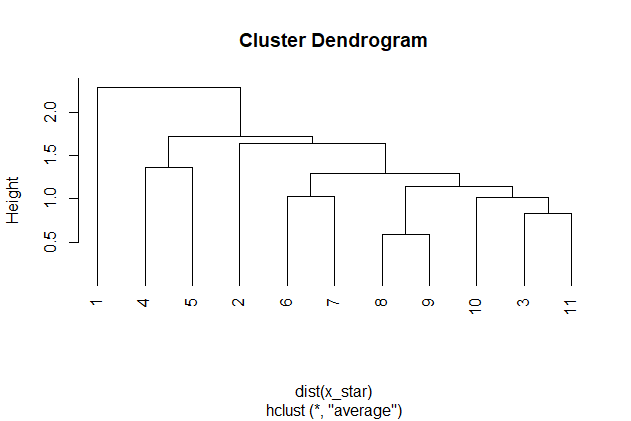
\includegraphics[width=11.5cm]{P3F4}
	\caption{数据归一化后进行R型聚类结果} \label{P3F3}
\end{figure}
\begin{figure}[h]
	\small
	\centering
	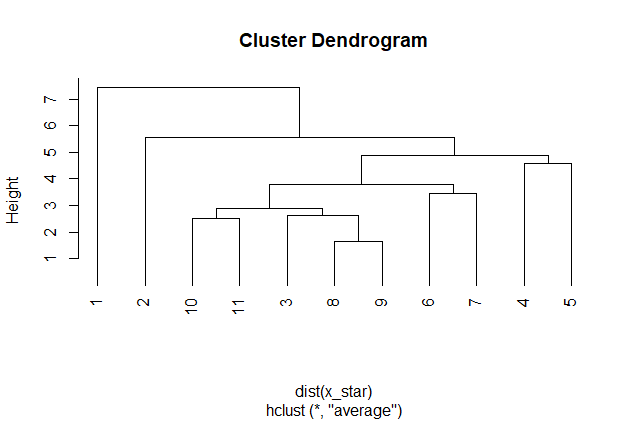
\includegraphics[width=11.5cm]{P3F3}
	\caption{数据标准化后进行R型聚类结果} \label{P3F4}
\end{figure}

从图\ref{P3F3}与图\ref{P3F4}可以看出,指标8 9 10 11具有较大的相关性,最先被聚到了一起。将18个指标 分为 6类,每一具体指标以及最终所确定的6个代表性指标如表\ref{P3T3}所示

\begin{table}[h]
	\centering
	\caption{各类别指标基本信息} \label{P3T3}
	\begin{tabular}{lll}
		\hline
		\textbf{序号} & \textbf{指标} & \textbf{代表类指标} \\ \hline
		第一类         & 1           & 感染人数           \\
		第二类         & 4           & 死亡率            \\
		第三类         & 5           & $R_0$             \\
		第四类         & 2           & 死亡人数           \\
		第五类         & 6 7         & 潜伏期            \\
		第六类         & 3 8 9 10 11 & 爆发地 治愈人数       \\ \hline
	\end{tabular}
\end{table}
从以上结果可以看出,指标 1(感染人数)、4(病死率),5($R_0$),2(死亡人数)与其它类型病症存在区别,各自单独为一类;第六类包含的指标较多 3(治愈率)、8(无症状感染者比例)、 9(持续时间)、11(爆发地信息),说明这几类指标具有一定的内在联系。一般来说,基本传染数和病死率直接影响传染病的危害程度,暴发地防疫措施与传染病持续时间有关。这些认识在分类结果中均有体现,这也说明了结果对于该问题具有较好的适应性。

\subsubsection{Q型聚类模型建立}
根据上述得出的结论,利用 Q 型聚类分析对 15 类经典传染病进行分类。

1. \textbf{样本的相似性度量}

要用数量化的方法对事物进行分类,就必须用数量化的方法描述事物之间的相似程度。对于待分类的样本点需用$p$个变量描述,故每个样本点可以看成是$R_p$空间中的一个点。因此,很自然地想到可以用距离来度量样本点间的相似程度。 在此我采用闵式距离进行计算求解,闵式距离计算如下:
$$
\begin{aligned}
\centering
d_{ij}(q)=\left( \sum_{k=1}^p \left|X_{ik}-x_{jk}\right|^q \right)^{\frac{1}{q}}
\end{aligned}
$$
此处我们采用q=2即欧几里得距离

2. \textbf{类间的相似性度量}

我采用类间平均连接法进行系统聚类,类间平均连接法定义类间距离平方为两类中元素两两之间距离平方的平均值,对于任意类$G_k$与$G_r$ 相似度为:

$$
\begin{aligned}
\centering
D_{kr}^2=\frac{n_p}{n_r}D_{kp}^2+\frac{n_q}{n_r}D_{kq}^2
\end{aligned}
$$

与R型聚类代码相似(附录C 224-250行),得到如图\ref{sp1}结果
\begin{figure}[h]
	\small
	\centering
	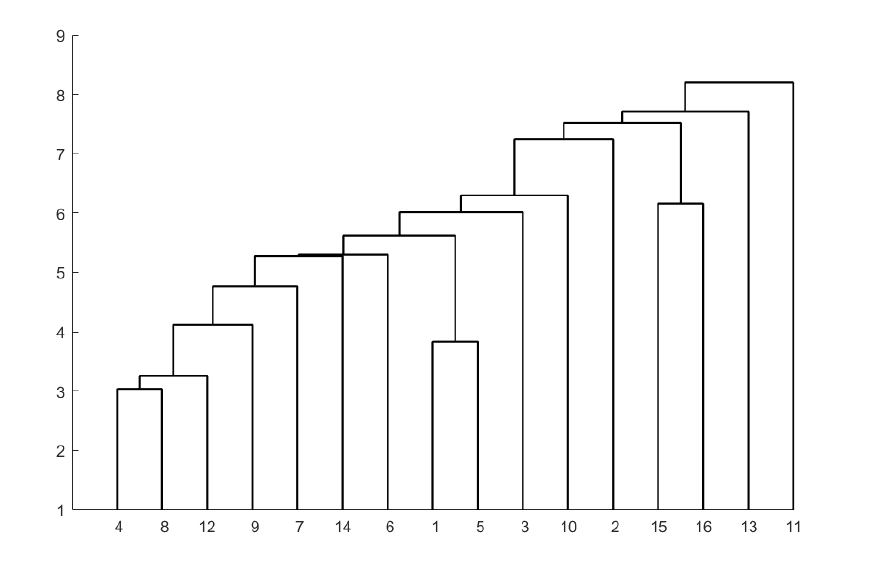
\includegraphics[width=11cm]{sp1}
	\caption{数据归一化后进行Q型聚类结果} \label{sp1}
\end{figure}
\begin{table}[H]
	\centering
	\caption{各类别病症基本信息} \label{P3T4}
	\begin{tabular}{llll}
		\hline
		\textbf{序号} & \textbf{传染病代号}          & \textbf{代表值} & \textbf{级别} \\ \hline
		第一类         & 11                      & 百日咳          & 散发          \\
		第二类         & 13                      & 腮腺炎          & 爆发          \\
		第三类         & 4,8,12,9,7,6,1,5,3,10,2 & 麻疹           & 流行          \\
		第四类         & 15,16                   & COVID-19     & 大流行         \\ \hline
	\end{tabular}
\end{table}
从图\ref{sp1},表\ref{P3T4}结果可以看出,传染病 11(百日咳)、13(腮腺炎)单独分为一类,传播级别分别为“散发”和“暴发”,传染病15(甲型H1N1)、16(COVID-19)分为一类,传播级别为“大流行”,第四类囊括了大部分的传染病(>50\%),传播级别为“流行”。通过查阅相关资料,百日咳是一种急性呼吸道传染病,但是很少能够通过外界条件传染,因此将其归为一类;而流行感冒能引起较大范围传播,但是传播途径易阻断(勤洗手、戴口罩),且病死率低,危害程度较小,归为一类;甲型 H1N1 和 COVID-19 传播能力强,患病致死率较高,传播途径较多,影响程度大,将其归为一类,其分类结果与世卫组织(WHO)给出的结论一致。这符合我们的认识,也说明了本模型具有较高的精度。 

\subsubsection{综合评价模型的建立}
\qquad 通过聚类分析将 16 类传染病分成了 4 类,并从 14 类指标中筛选出了6 类影响较大的指标。接下来,我们根据不同的类别,利用综合评价模型对不同类别的传染病进行打分,实现类别的定量划分。由于量化指标较多,数据较大,我们选用主成分分析模型作为传染病分类评价模型。评价指标有:感染人数,死亡率,$R_0$,死亡人数,潜伏期,爆发地,治愈人数

使用主成分分析法的标准方法:1. 数据标准化 2. 计算相关系数矩阵R 3. 求特征值与特征向量 4. 计算特征值的贡献率 5. 对不同传染病进行打分排序得到流行病判定的数学边界.最终得到主成分累计贡献值(附录C 252-293行),表\ref{P3T5}与图\ref{P3F5}

\begin{table}[H]
	\centering
	\caption{贡献率和累计贡献率结果} \label{P3T5}
	\begin{tabular}{llll}
		\hline
		\textbf{序号} & \textbf{特征值} & \textbf{贡献率} & \textbf{累计贡献率} \\ \hline
		1           & 44.1742      & 0.4417       & 0.4417         \\
		2           & 23.8824      & 0.2388       & 0.6806         \\
		3           & 16.3155      & 0.1632       & 0.8437         \\
		4           & 9.1831       & 0.0918       & 0.9356         \\
		5           & 4.7594       & 0.0486       & 0.9842         \\
		6           & 1.6052       & 0.0158       & 1              \\ \hline
	\end{tabular}
\end{table}

\begin{figure}[h]
	\small
	\centering
	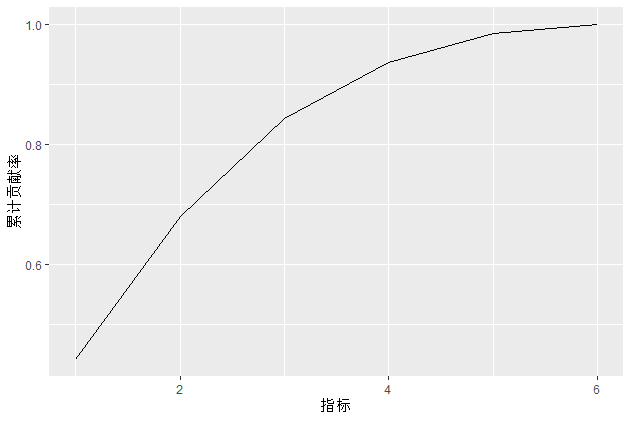
\includegraphics[width=12cm]{P3F5}
	\caption{主成分累计贡献率分布图} \label{P3F5}
\end{figure}
如表\ref{P3T5},图\ref{P3F5}可知P>=4时累计贡献率已经超过90\%,故使用前四组指标变量代替6个指标进行分析,易得主成分综合评价模型为:
\begin{table}[H]
	\centering
	\begin{tabular}{lll}
		\hline
		\textbf{序号} & \textbf{指标} & \textbf{代表类指标} \\ \hline
		第一类         & 1           & 感染人数           \\
		第二类         & 4           & 死亡率            \\
		第三类         & 5           & $R_0$             \\
		第四类         & 2           & 死亡人数           \\ \hline
	\end{tabular}
\end{table}
$$
Z=0.4417y_1+0.2388y_2+0.1632y_3+0.0918y_4
$$

根据对评分结果进行归一化处理,得到了四种类别综合得分,绘制得分分布图如图\ref{P3F6}:
\begin{figure}[H]
	\small
	\centering
	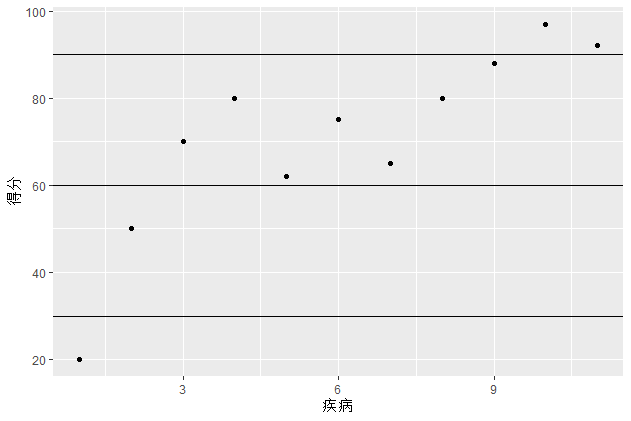
\includegraphics[width=12cm]{P3F6}
	\caption{各类传染病综合得分结果分布} \label{P3F6}
\end{figure}
	
我们可以看出归一化得分在区间[0,30]时对应的传播类型为“散发”,归一化得分在区间(30,60]时对应的传播类型为“暴发”,归一化得分在区间(60,90]时对应的传播类型为“流行”,归一化得分在区间(90,100]时对应的传播类型为“大流行”。问题一中所述的传染病均为传播较为广泛的疾病,其中甲型 H1N1 和 COVID-19给人类经济生产带来的影响最大,因此被归纳为“大流行”传播级别。这一分类结果符合我们的认识,具有一定的合理性。


\subsection{使用改进SEIR模型预测无症状感染者数目}
病毒传播动力学模型一般有多群体传播的S-DI-A模型,具有脉冲的SIS传染病模型,常微分方程的SIQS,SEIR模型,具有时滞的SIRS模型。我选用了较为通用的SEIR模型

1.\textbf{SI模型}
\begin{figure}[H]
	\small
	\centering
	
\includegraphics[width=8.5cm]{C1}
	\caption{SI模型} \label{C1}
\end{figure}
SI模型把人群分为2种,一种是易感者,易感者是健康的人群,用$S$表示其人数,另外一种是感染者,即患者,人数用$I$来表示。我们假设一个区域内总人数是$N$则$N=S+I$,若$I$个感染者没有被有效隔离,每人每天遇到r人,有$\beta$的概率会传染,健康人的比例为$\frac {S}{N}$ ,将上述变量相乘即为每日新增病例数,微分方程形式如下
$$
\begin{aligned}
\frac{dI}{dt}&=\frac{r\beta IS}{N}    \\
\frac{dS}{dt}&=-\frac{r\beta IS}{N}
\end{aligned}
$$
可以使用R语言轻松对预测值计算
$$
\begin{aligned}
I_n&=I_{n-1}+\frac{r\beta {I_n}-1S{n-1}}{N}    \\
S_n&=S_{n-1}-\frac{r\beta {	I_n}-1S{n-1}}{N}
\end{aligned}
$$

2.\textbf{SIS模型}
\begin{figure}[H]
	\small
	\centering
	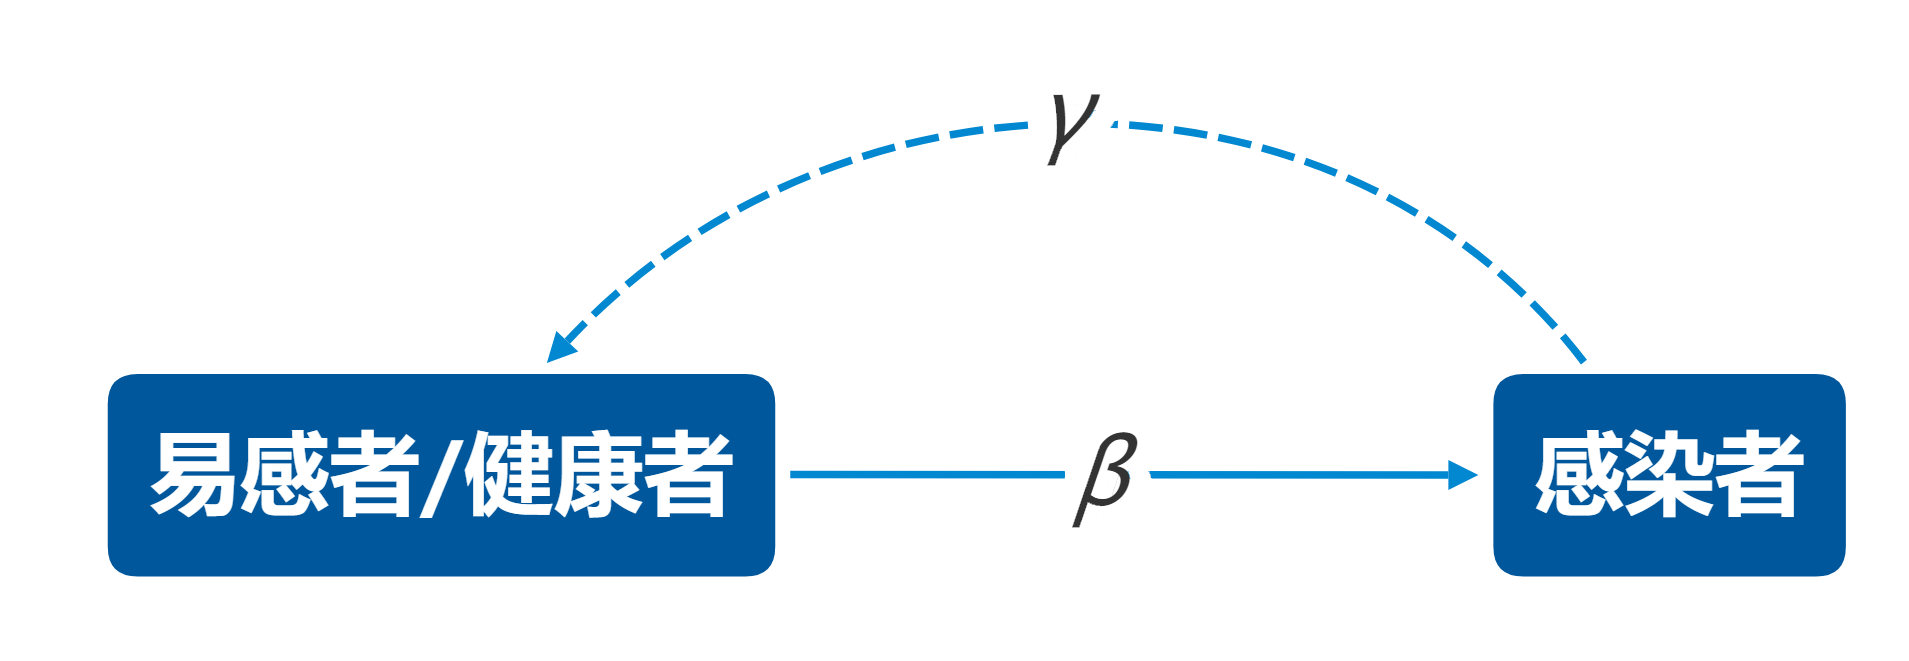
\includegraphics[width=8.5cm]{C2}
	\caption{SIS模型} \label{C2}
\end{figure}
对SI模型进行改进,认为有的人治好了但是还会反复感染,类似与流感的传播。

这样子的模型就是SIS模型,SIS模型比SI模型多了一个感染者$I$恢复健康的概率$\gamma$ 。再次加入到微分方程中:
$$
\begin{aligned}
\frac{dI}{dt}&=\frac{r\beta IS}{N}-\gamma I\\
\frac{dS}{dt}&=-\frac{r\beta IS}{N}+\gamma I\\
\end{aligned}
$$

迭代方程修改为

$$
\begin{aligned}
I_n&=I_{n-1}+\frac{r\beta I_{n-1}S_{n-1}}{n}-\gamma I  \\
S_n&=S_{n-1}-\frac{r\beta I_{n-1}S_{n-1}}{n}+\gamma I
\end{aligned}
$$

3.\textbf{SIR模型}
\begin{figure}[H]
	\small
	\centering
	
\includegraphics[width=11cm]{C3}
	\caption{SIR模型} \label{C3}
\end{figure}

对SI模型进行改进,考虑人在康复以后产生了抗体就不会再得病。不同于SIS模型,我们在模型中引入康复者,用 R表示,并满足总人数N=S+I+R。这个时候就是SIR模型。一旦变为康复者,就不会再传染,即在概率传递过程中,一旦变为康复者,就没有概率再次转移为感染者或者易感者。我们假设感染者变为康复者的概率为$\gamma $, 同样列出微分方程:
$$
\begin{aligned}
\frac{dS}{dt}&=\frac{-r\beta IS}{N}  \\
\frac{dI}{dt}&=\frac{r\beta IS}{N}-\gamma I \\
\frac{dR}{dt}&=\gamma I
\end{aligned}
$$

迭代方程为:

$$
\begin{aligned}
S_n&=S_{n-1}-\frac{r\beta I_{n-1}S_{n-1}}{N}  \\
I_n&=I_{n-1}+\frac{r\beta I_{n-1}S_{n-1}}{N}-\gamma I_{n-1}  \\
R_n&=R_{n-1}+\gamma I_{n-1}
\end{aligned}
$$

4.\textbf{SEIR模型}
\begin{figure}[H]
	\small
	\centering
	
\includegraphics[width=13cm]{C4}
	\caption{SEIR模型} \label{C4}
\end{figure}

实际情况更加复杂,易感染人群在一开始会经历潜伏期(无症状感染期),一段时间之后才出现症状,因此我们在SIR模型的基础上引入了潜伏者(无症状感染者),潜伏者按照概率$\alpha$转化为感染者,在SIR的基础上修改微分方程:
$$
\begin{aligned}
\frac{dS}{dt}&=-\frac{r\beta IS}{N}\\ 
\frac{dE}{dt}&=\frac{r\beta IS}{N}-\alpha E\\ 
\frac{dI}{dt}&=\alpha E-\gamma I\\ 
\frac{dR}{dt}&=\gamma I
\end{aligned}
$$

迭代方程为:

$$
\begin{aligned}
S_n&=S_{n-1}-\frac{r\beta I_{n-1}S_{n-1}}{N}\\ 
E_n&=E_{n-1}+\frac{r\beta I_{n-1}S_{n-1}}{N}-\alpha E_{n-1}\\ 
I_n&=I_{n-1} +\alpha E_{n-1}-\gamma I_{n-1}\\ 
R_n&=R_{n-1}+\gamma I_{n-1}
\end{aligned}
$$

\subsubsection{对SEIR模型在COVID-19中的改进(以重庆为例)}
我们发现在COVID-19疫情中,无症状感染者(潜伏者)在病毒潜伏期具有传染性,因此我们要引入潜伏者的传染概率$\beta_2$可以将健康的人群转变为无症状感染者(潜伏者)。而无症状感染者每天接触的健康易感者人数为$r_2$。得到微分方程为:

$$
\begin{aligned}
	\frac{dS}{dt}&=-\frac{r\beta IS}{N}-\frac{r_2 \beta_2ES}{N} \\
	\frac{dE}{dt}&=\frac{r\beta IS}{N}-\alpha E+\frac{r_2 \beta_2ES}{N}  \\ 
	\frac{dI}{dt}&=\alpha E-\gamma I  \\ 
	\frac{dR}{dt}&=\gamma I
\end{aligned}
$$
得到迭代方程:

$$
\begin{aligned}
S_n&=S_{n-1}-\frac{r\beta I_{n-1}S_{n-1}}{N}-\frac{r_2\beta_2 E_{n-1}S_{n-1}}{N}  \\
E_n&=E_{n-1}+\frac{r\beta I_{n-1}S_{n-1}}{N}-\alpha E_{n-1}+\frac{r_2\beta_2 E_{n-1}S_{n-1}}{N}  \\ 
I_n&=I_{n-1} +\alpha E_{n-1}-\gamma I_{n-1}  \\ 
R_n&=R_{n-1}+\gamma I_{n-1}
\end{aligned}
$$
我们将重庆市的感染人数数据代入模型发现无论如何修改参数,预报值在初始几日与实际值差距较小,但是随着时间延长差距变大,我认为是因为:1. 模型中的$S$为易感者而非所有人口。 2. 当病毒在某城市大规模爆发之后城市会采取防疫措施,此时$r$与$r_2$值会瞬间下降。 3. 康复率随着时间而升高(若借鉴了其他城市的经验则会瞬间升高)。于是加入两条件再次预测(附录C 296-343行)结果如图\ref{P3F7}

\begin{figure}[H]
	\small
	\centering
	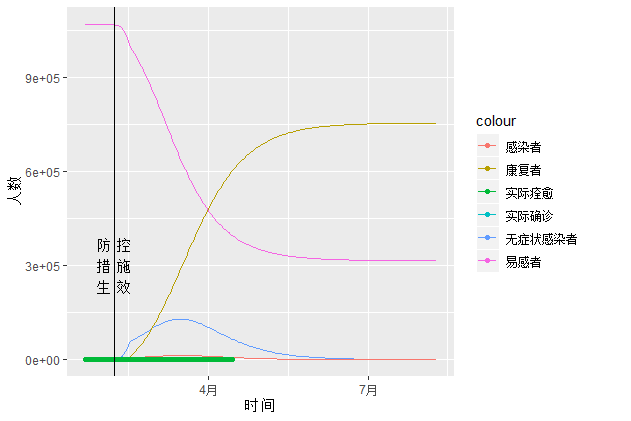
\includegraphics[width=15cm]{P3F7}
	\caption{对SEIR模型第一次改进的预测结果} \label{P3F7}
\end{figure}

实际数据与预测数据相差仍然很大,阅读他人预测论文后我发现预测偏差原因为 1. 部分易感者与无症状感染者采取了自我隔离 2. 存在患者在潜伏期与发病期自愈,即SEIR模型应修正为图\ref{C5}:

\begin{figure}[H]
	\small
	\centering
	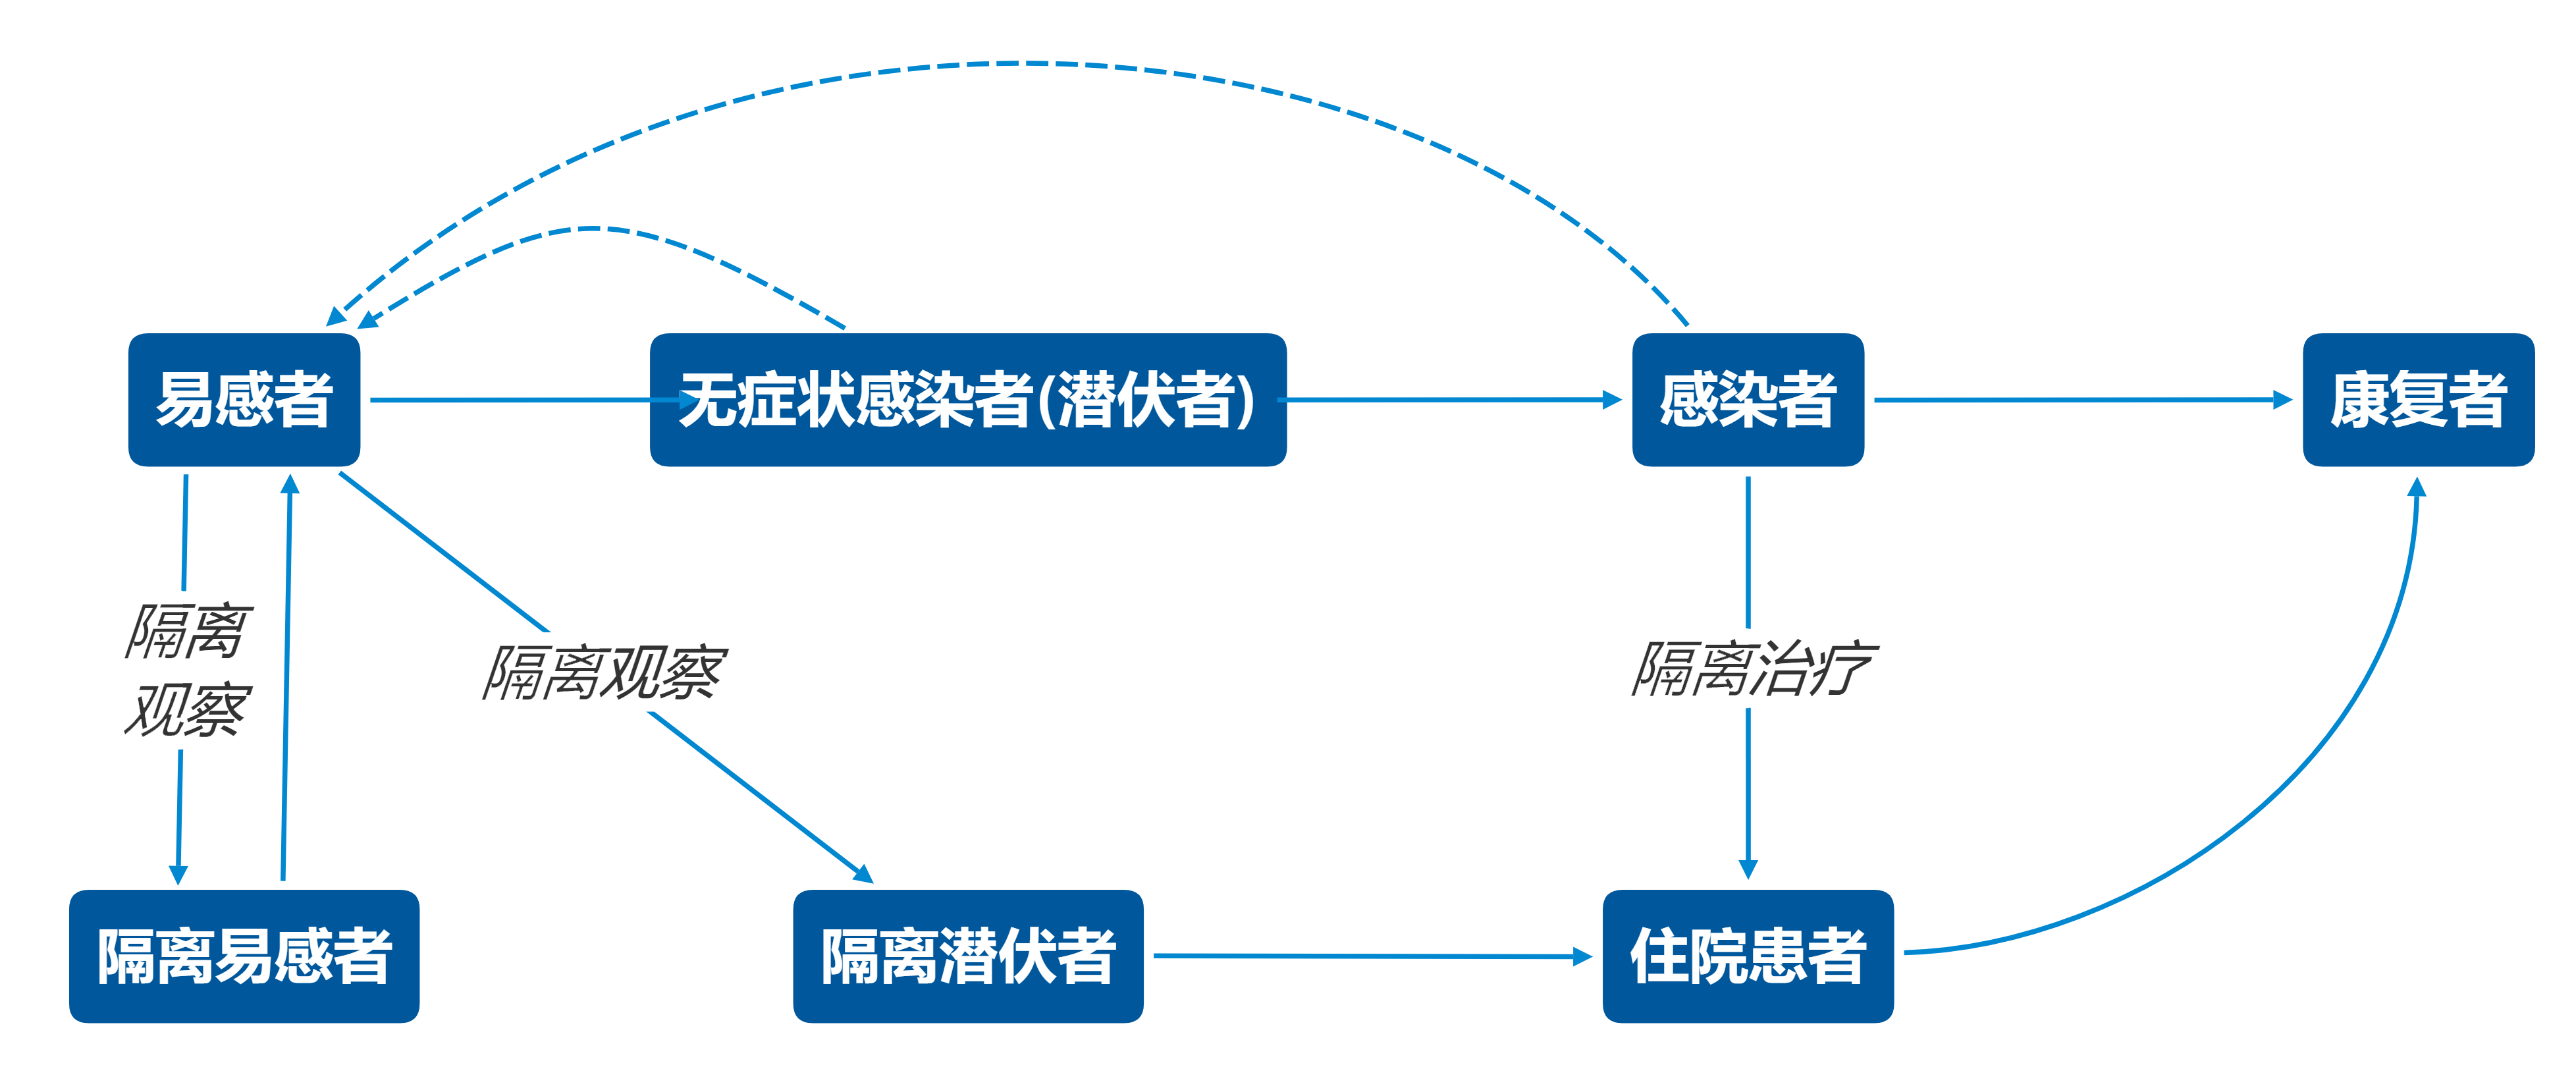
\includegraphics[width=14cm]{C5}
	\caption{SEIR模型第二次改进} \label{C5}
\end{figure}

假设隔离比例为$q$,传染概率为$\beta$,接触率为$c$,$\rho$是有效接触系数,有效接触系数的参考值取1,$\rho  c$ 是有效接触率。易感者 $S$ 向隔离易感者$S_q$、隔离潜伏者$E_q$、潜伏者 $E$ 的转化速率为$\rho c q(1-\beta)$,$\rho c q \beta$和 $\rho c \beta (1-q)$ 。同时考虑到非隔离的感染者 $I$ 和潜伏者 $E$ 对易感人群的影响,又有隔离解除的易感者 $S_q$重新转变为 $S$,因此易感者人数控制方程为

$$
\frac{dS}{st}=S(1+\theta E)\left[ \rho c \beta + \rho cq(1-\beta) \right]+\lambda S_q
$$

其中$\theta$是无症状感染者相对于一般感染者传播能力的比值,我们假设在病毒传播最开始时传播能力相同,即$\theta =1$。$\lambda$ 是隔离解除速率,取$\lambda=\frac{1}{14}$(隔离时长为14天)。于是构建新的SEIR模型的微分方程:

$$
\begin{aligned}
\frac{dS}{st}&=S(1+\theta E)\left[ \rho c \beta + \rho cq(1-\beta) \right]+\lambda S_q \\
\frac{dE}{dt}&=\rho c \beta (1-q)S(I+\theta E)-\sigma E \\
\frac{dI}{dt}&=\sigma E-\left( \delta_I +\alpha +\gamma_I \right)I \\
\frac{dS_q}{dt}&=\rho c q(1-\beta)S(I+\theta E)-\lambda S_q \\
\frac{dE_q}{dt}&=\rho c \beta q S(I+\theta E)-\delta_qE_q \\
\frac{dH}{dt}&=\delta_II+\delta_qE_q-\left( \alpha + \gamma_H \right)H \\
\frac{dR}{dt}&=\gamma_II+\gamma_HH
\end{aligned}
$$

我使用重庆市数据作为查询集了解不同参数对于结果图像变化进行分析,得到参数具体值(附录C 364-376行)。将湖北省感染人数数据作为测试集进行测试(附录C 347-425行)得到图\ref{P3F8},图\ref{P3F9}

\begin{figure}[H]
	\small
	\centering
	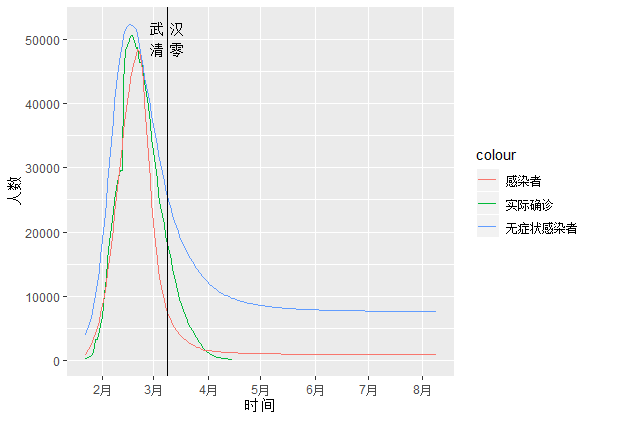
\includegraphics[width=12.5cm]{P3F8}
	\caption{SEIR模型第二次改进后的感染人数与实际人数进行比较并预测无症状感染人数} \label{P3F8}
\end{figure}

\begin{figure}[H]
	\small
	\centering
	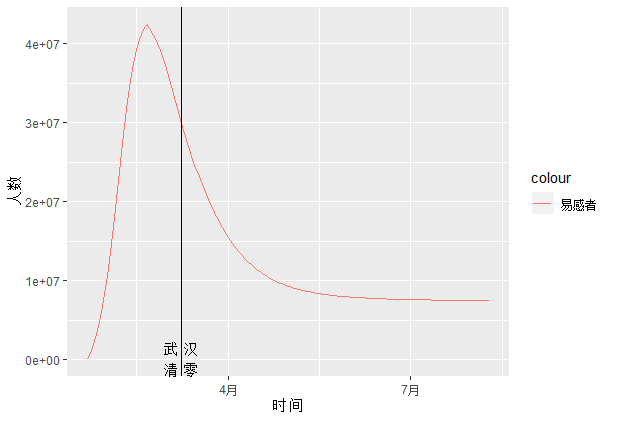
\includegraphics[width=12.5cm]{P3F9}
	\caption{对SEIR模型第二次改进后易感人数变化} \label{P3F9}
\end{figure}

\subsubsection{结果分析}
可以看出,该曲线共分为三个阶段。第一阶段是早期上升阶段:属于病毒暴发早期,潜伏者(无症状感染人数)人数快速上升,由无症状感染者人数也持续上升;第二阶段为中期调控阶段,该阶段一开始实行了封城隔离、佩戴口罩、治疗等措施,无症状人数虽有上升,但是后期得到了控制,大约22 天后达到了峰值;第三阶段为后期下降阶段,该阶段由于前面的措施持续进行,无症状感染人数下降趋势明显,在疫情开始后的140 天内,日新增无症状感染者人数降为0,也就是说,大约到5 月中旬,湖北地区的新增无症状感染人数会趋近于0。
无症状感染者人数在2020年4月15-2020年8月9日无症状感染者人数预测为附录B

\subsection{使用响应面预测模型验证SEIR模型}
在无症状感染者人数变化趋势时我们使用的SEIR模型属于病毒传播动力学模型,我们还可以通过统计学模型预测无症状感染者人数,于是我采用响应面预测模型预测无症状感染者人数从而对改进SEIR模型进行验证

我以无症状感染人数 Y 为因变量,根据 R 型聚类结果选取 4 种典型指标:患病人数 P、基本传染数 $R_0$、潜伏期 T、治愈率 $R_c$ 四个指标。为预测无症状感染人数发展趋势,我们拟采用响应面预测模型,建立 Y 与四个指标的关系式。 

响应面设计方法, 通过设计合理的试验方法并通过合理的操作得到试验结果数据,采用多元二次线性回归方法建立自变量和响应值之间的函数关系,通过回归方程来分析响应值的变化趋势,该方法在解决多变量问题中较为常见。 

由于R语言实现响应面预测是否复杂,我使用了实验设计软件 Design-Expert,选用 BBD 实验设计方法。响应面指响应变量(因变量)Y 与一组输入变量$x_i$的函数关系式。

实验中响应变量指无症状感染人数 Y,自变量考虑了 P、$R_0$、T 和 $R_c$ 四个因素。Design-Expert共进行了 29 组实验,获得表\ref{P3T8}
\vspace{-0.5cm}
\begin{table}[H]
	\centering
	\caption{效果最好的五个实验} \label{P3T8}
	\begin{tabular}{llllll}
		\hline
		\textbf{项目} & \textbf{P} & \textbf{$R_0$} & \textbf{T} & \textbf{$R_c$} & \textbf{Y} \\ \hline
		实验一         & 2.75       & 5              & 12.5       & 0.2            & 2202       \\
		实验二         & 5          & 3              & 12.5       & 1              & 1971       \\
		实验三         & 0.5        & 3              & 20         & 0.6            & 1325       \\
		实验四         & 0.5        & 3              & 5          & 0.6            & 883        \\
		实验五         & 2.75       & 3              & 12.5       & 0.6            & 1243
		\\ \hline
	\end{tabular}
\end{table}

于是我们建立响应面二次多项式模型
$$
\begin{aligned}
y=1.65+0.35P+0.57R_0+0.1T-0.55R_c+0.16PR_0-0.11PT+0.15PR_c \\
-0.04R_0T+0.14R_0R_c+0.02P^2+0.09R_0^2-0.18T^2-0.05R_c^2
\end{aligned}
$$

在响应面分析过程中,用 F 值进行统计结果的显著性检测,利用 p 值来检测回归系数的显著性,p 值越小,表明结果越显著。结果如表所示。由表\ref{P3T9}可得,模型F值为 5.37,p<0.05,说明模型具有显著的适应性,回归方程中各因素与响应值之间的关系是显著。

\begin{table}[h]
	\centering
	\caption{响应面分析表} \label{P3T9}
	\begin{tabular}{llllll}
		\hline
		\textbf{参数}  & \textbf{平方和} & \textbf{自由度} & \textbf{均方} & \textbf{F 值} & \textbf{p 值}     \\ \hline
		\textbf{模型}  & 9.84         & 14           & 0.70        & 5.37         & 0.0017(显著)       \\
		\textbf{A}   & 1.48         & 1            & 1.48        & 11.29        & 0.0047           \\
		\textbf{B}   & 3.91         & 1            & 3.91        & 29.93        & \textless 0.0001 \\
		\textbf{C}   & 0.13         & 1            & 0.13        & 0.98         & 0.3387           \\
		\textbf{D}   & 3.68         & 1            & 3.68        & 28.10        & 0.0001           \\
		\textbf{残差}  & 1.83         & 14           & 0.13        &              &                  \\
		\textbf{净误差} & 0.23         & 4            & 0.059       &              &                  \\
		\textbf{总误差} & 11.67        & 28           &             &              &                  \\ \hline
	\end{tabular}
\end{table}

画出无症状感染者随时间变化数目图像如图\ref{res}:

\begin{figure}[H]
	\small
	\centering
	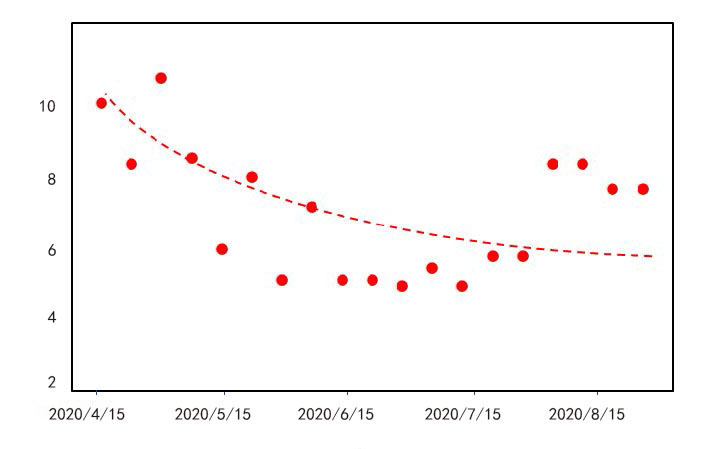
\includegraphics[width=11cm]{res}
	\caption{对无症状感染者人数的预测} \label{res}
\end{figure}

至此我们验证了改进SEIR模型的正确性!

这场席卷全球的灾难让我们重新认识了我们的自信、坚毅,意志、守望相助...数据科学家在第一时间使用各种模型预测了病毒的发展趋势,为疫情防控起到了重要指导作用。但最重要的是,\textbf{我们坚信没有任何困难能够将我们击败,坚信冰雪终将消融,春天也会如期而至,我们的国家春暖花开、否极泰来。}

\newpage
\begin{thebibliography}{99}
	\addcontentsline{toc}{subsection}{参考文献}
	\bibitem{1}Weiss, R. A., \& McMichael, A. J. (2004). Social and environmental risk factors in the emergence of infectious diseases. Nature medicine, 10(12 Suppl), S70–S76. https://doi.org/10.1038/nm1150
	\bibitem{2}Tang, B., Wang, X., Li, Q., Bragazzi, N. L., Tang, S., Xiao, Y., \& Wu, J. (2020). Estimation of the Transmission Risk of the 2019-nCoV and Its Implication for Public Health Interventions. Journal of clinical medicine, 9(2), 462. https://doi.org/10.3390/jcm9020462
	\bibitem{3}Wu, J. T., Leung, K., \& Leung, G. M. (2020). Nowcasting and forecasting the potential domestic and international spread of the 2019-nCoV outbreak originating in Wuhan, China: a modelling study. The Lancet, 395(10225), 689-697.
	\bibitem{4}Weiss RA, McMichael AJ. Social and environmental risk factors in the emergence of infectious diseases. Nature Medicine. 2004 Dec;10(12 Suppl):S70-6. DOI: 10.1038/nm1150.
	\bibitem{5}Mutreja, A., Kim, D. W., Thomson, N. R., Connor, T. R., Lee, J. H., Kariuki, S., ... \& Niyogi, S. K. (2011). Evidence for several waves of global transmission in the seventh cholera pandemic. Nature, 477(7365), 462-465.
	\bibitem{6}Murray, C. J., Lopez, A. D., Chin, B., Feehan, D., \& Hill, K. H. (2006). Estimation of potential global pandemic influenza mortality on the basis of vital registry data from the 1918–20 pandemic: a quantitative analysis. The Lancet, 368(9554), 2211-2218.
	\bibitem{7}World Health Organization. 2018. Pandemic Preparedness. [online] Available at: <https://www.who.int/influenza/preparedness/pandemic/en/> [Accessed 13 June 2020].
	\bibitem{8}Hou, C., Chen, J., Zhou, Y., Hua, L., Yuan, J., He, S., ... \& Zhang, J. (2020). The effectiveness of quarantine of Wuhan city against the Corona Virus Disease 2019 (COVID‐19): A well‐mixed SEIR model analysis. Journal of medical virology.
	\bibitem{9}Zou, Y., Pan, S., Zhao, P., Han, L., Wang, X., Hemerik, L., ... \& van der Werf, W. (2020). Outbreak analysis with a logistic growth model shows COVID-19 suppression dynamics in China. medRxiv.

\end{thebibliography}


\newpage
\subsection*{附录}
\addcontentsline{toc}{subsection}{附录}
\subsubsection*{附录 A: 15种常见传染病大爆发汇总}

\begin{table}[H]
	\begin{tabular}{llllll}
		\hline
		\textbf{疾病名} & \textbf{感染数} & \textbf{死亡数} & \textbf{治愈数} & \textbf{死亡率} & \textbf{$R_0$小值} \\ \hline
		乙肝           & 300000000    & 17000        & 2999998300   & 0.000005     & 1                \\
		黑死病          & 85000000     & 78700000     & 6300000      & 0.9258       & 1                \\
		霍乱           & 461783       & 8072         & 453711       & 0.0068       & 1                \\
		麻疹           & 250270       & 5110         & 245160       & 0.0020       & 12               \\
		白喉           & 2839         & 67           & 2772         & 0.0235       & 6                \\
		天花           & 6000         & 850          & 5150         & 0.3          & 5                \\
		骨髓灰质炎        & NA           & NA           & NA           & NA           & 5                \\
		风疹           & NA           & NA           & NA           & 0.0013       & 5                \\
		腮腺炎          & NA           & NA           & NA           & 0.0002       & 5                \\
		艾滋病          & NA           & NA           & NA           & NA           & 2                \\
		获得性免疫缺陷综合征   & 75598200     & 5292         & 75592908     & 0.00007      & 4                \\
		非典           & 8422         & 919          & 7503         & 0.17         & 0.85             \\
		中东呼吸综合征      & 1139         & 431          & 708          & 0.37         & 1                \\
		甲型HIN1流感     & 25449514     & 19449        & 25430065     & 0.012        & 1.75             \\
		新型冠状肺炎       & 7221717      & 411818       & 6809899      & 0.05         & 3.77             \\ \hline
	\end{tabular}
\end{table}

\begin{table}[H]
	\begin{tabular}{llllll}
		\hline
		\textbf{疾病名} & \textbf{$R_0$大值} & \textbf{潜伏期} & \textbf{无症状感染者比例} & \textbf{持续时间} & \textbf{传播国家} \\ \hline
		乙肝           & 2                & 70           & NA                & NA            & 1               \\
		黑死病          & 3                & 3            & 0.12              & 2555          & 1               \\
		霍乱           & 2                & 2            & 0.07              & 1277          & 1               \\
		麻疹           & 18               & 10           & 0.08              & 317           & 0.025           \\
		白喉           & 7                & 3            & 0.11              & 115           & 0.01            \\
		天花           & 7                & 14           & NA                & 730           & 1               \\
		骨髓灰质炎        & 7                & 11           & NA                & NA            & 1               \\
		风疹           & 7                & 11           & 0.01              & NA            & NA              \\
		腮腺炎          & 7                & 19           & 0.06              & NA            & NA              \\
		艾滋病          & 5                & 11           & 0.04              & NA            & 1               \\
		获得性免疫缺陷综合征   & 7                & 13           & 0.09              & NA            & 1               \\
		非典           & 3                & 7            & 0.11              & 270           & 0.162           \\
		中东呼吸综合征      & 2                & 5.2          & 0.18              & 218           & 0.061           \\
		甲型HIN1流感     & 1.75             & 4            & 0.19              & 485           & 1               \\
		新型冠状肺炎       & 3.77             & 14           & 0.17              & 190           & 1               \\ \hline
	\end{tabular}
\end{table}
\begin{table}[H]
	\begin{tabular}{lllll}
		\hline
		\textbf{疾病名} & \textbf{始发地人口} & \textbf{始发地经济} & \textbf{始发地人口密度} & \textbf{防控程度} \\ \hline
		乙肝           & NA             & NA             & NA               & NA            \\
		黑死病          & 70000000       & NA             & 16               & 0             \\
		霍乱           & 7510100        & 3894           & 554              & NA            \\
		麻疹           & 1800000        & 3198           & NA               & NA            \\
		白喉           & 257740000      & 3894           & 554              & NA            \\
		天花           & 11000          & NA             & NA               & NA            \\
		骨髓灰质炎        & NA             & NA             & NA               & NA            \\
		风疹           & NA             & NA             & NA               & NA            \\
		腮腺炎          & NA             & NA             & NA               & NA            \\
		艾滋病          & NA             & NA             & NA               & NA            \\
		获得性免疫缺陷综合征   & NA             & NA             & NA               & NA            \\
		非典           & 7251900        & 7404           & 975              & NA            \\
		中东呼吸综合征      & 436000         & 25059          & 965              & NA            \\
		甲型HIN1流感     & 38310000       & 49911          & 90               & NA            \\
		新型冠状肺炎       & 12212000       & 21098          & 2334             & 1             \\ \hline
	\end{tabular}
\end{table}

\newpage
\subsubsection*{附录 B: 改进SEIR模型对武汉无症状感染者人数的预测}
\begin{table}[H]
	\begin{tabular}{llllllll}
		\hline
		日期        & 人数       & 日期        & 人数       & 日期        & 人数       & 日期        & 人数       \\ \hline
		2020/4/15 & 9725     & 2020/5/15 & 8174.533 & 2020/6/14 & 7819.946 & 2020/7/14 & 7699.848 \\
		2020/4/16 & 9620.579 & 2020/5/16 & 8153.683 & 2020/6/15 & 7813.932 & 2020/7/15 & 7697.225 \\
		2020/4/17 & 9522.292 & 2020/5/17 & 8133.799 & 2020/6/16 & 7808.122 & 2020/7/16 & 7694.655 \\
		2020/4/18 & 9429.725 & 2020/5/18 & 8114.827 & 2020/6/17 & 7802.507 & 2020/7/17 & 7692.136 \\
		2020/4/19 & 9342.496 & 2020/5/19 & 8096.72  & 2020/6/18 & 7797.078 & 2020/7/18 & 7689.667 \\
		2020/4/20 & 9260.251 & 2020/5/20 & 8079.431 & 2020/6/19 & 7791.826 & 2020/7/19 & 7687.244 \\
		2020/4/21 & 9182.666 & 2020/5/21 & 8062.917 & 2020/6/20 & 7786.742 & 2020/7/20 & 7684.867 \\
		2020/4/22 & 9109.437 & 2020/5/22 & 8047.137 & 2020/6/21 & 7781.819 & 2020/7/21 & 7682.533 \\
		2020/4/23 & 9040.285 & 2020/5/23 & 8032.052 & 2020/6/22 & 7777.05  & 2020/7/22 & 7680.241 \\
		2020/4/24 & 8974.952 & 2020/5/24 & 8017.626 & 2020/6/23 & 7772.428 & 2020/7/23 & 7677.989 \\
		2020/4/25 & 8913.197 & 2020/5/25 & 8003.825 & 2020/6/24 & 7767.945 & 2020/7/24 & 7675.775 \\
		2020/4/26 & 8854.796 & 2020/5/26 & 7990.615 & 2020/6/25 & 7763.597 & 2020/7/25 & 7673.599 \\
		2020/4/27 & 8799.543 & 2020/5/27 & 7977.968 & 2020/6/26 & 7759.375 & 2020/7/26 & 7671.459 \\
		2020/4/28 & 8747.245 & 2020/5/28 & 7965.853 & 2020/6/27 & 7755.275 & 2020/7/27 & 7669.352 \\
		2020/4/29 & 8697.721 & 2020/5/29 & 7954.243 & 2020/6/28 & 7751.292 & 2020/7/28 & 7667.279 \\
		2020/4/30 & 8650.805 & 2020/5/30 & 7943.114 & 2020/6/29 & 7747.42  & 2020/7/29 & 7665.237 \\
		2020/5/1  & 8606.34  & 2020/5/31 & 7932.44  & 2020/6/30 & 7743.655 & 2020/7/30 & 7663.226 \\
		2020/5/2  & 8564.181 & 2020/6/1  & 7922.198 & 2020/7/1  & 7739.99  & 2020/7/31 & 7661.245 \\
		2020/5/3  & 8524.192 & 2020/6/2  & 7912.367 & 2020/7/2  & 7736.424 & 2020/8/1  & 7659.292 \\
		2020/5/4  & 8486.246 & 2020/6/3  & 7902.926 & 2020/7/3  & 7732.95  & 2020/8/2  & 7657.366 \\
		2020/5/5  & 8450.224 & 2020/6/4  & 7893.856 & 2020/7/4  & 7729.565 & 2020/8/3  & 7655.466 \\
		2020/5/6  & 8416.015 & 2020/6/5  & 7885.138 & 2020/7/5  & 7726.265 & 2020/8/4  & 7653.592 \\
		2020/5/7  & 8383.515 & 2020/6/6  & 7876.755 & 2020/7/6  & 7723.046 & 2020/8/5  & 7651.742 \\
		2020/5/8  & 8352.626 & 2020/6/7  & 7868.691 & 2020/7/7  & 7719.906 & 2020/8/6  & 7649.916 \\
		2020/5/9  & 8323.258 & 2020/6/8  & 7860.929 & 2020/7/8  & 7716.84  & 2020/8/7  & 7648.113 \\
		2020/5/10 & 8295.325 & 2020/6/9  & 7853.456 & 2020/7/9  & 7713.846 & 2020/8/8  & 7646.331 \\
		2020/5/11 & 8268.746 & 2020/6/10 & 7846.257 & 2020/7/10 & 7710.921 & 2020/8/9  & 7644.571 \\
		2020/5/12 & 8243.446 & 2020/6/11 & 7839.318 & 2020/7/11 & 7708.061 &           &          \\
		2020/5/13 & 8219.354 & 2020/6/12 & 7832.628 & 2020/7/12 & 7705.264 &           &          \\
		2020/5/14 & 8196.404 & 2020/6/13 & 7826.174 & 2020/7/13 & 7702.527 &           &          \\ \hline
	\end{tabular}
\end{table}

\newpage
\subsubsection*{附录 C:源代码}
\begin{minted}%
[encoding=utf8,
linenos,
frame=single,
rulecolor=purple!50!black,
texcl=true,
highlightcolor=green!40,
breaklines=true,
]{R}
library(tidyverse)
library(purrr)
library(psych)

#-----------------------------------------------------------------------
#     3.3 数据预处理
#-----------------------------------------------------------------------

# 若使用Rpeoject打开则无需手动设置工作路径
# setwd("C:/Users/tclkr/Desktop/COVID19")

data_state_local<-read.csv("../data/reference.csv")
data_state_number<-read.csv("../data/time-series-19-covid-combined.csv")
data_us_confirmed<-read.csv("../data/us_confirmed.csv")
data_us_die<-read.csv("../data/us_deaths.csv")
data_world_summary<-read.csv("../data/worldwide-aggregated.csv")

get_key<-function(a,b){
  if(a==''){
  # 遇到一个bug,但是这样复杂一点就能运行
    return(paste(b))
  }
  return(paste(a,sep =" ,",b))
}

## 数据清洗
### 世界各国(省)数据
data_state_local$Combined_Key=as.character(data_state_local$ Combined_Key)
data_glb<-data_state_number%>%
# num的经纬度精度不如local的好
select(-Long,-Lat)%>%
  mutate(Combined_Key = purrr::map2_chr(Province.State,Country.Region,get_key))

# 清洗主键
data_state_local$Combined_Key<-gsub(" , ",",",data_state_local$Combined_Key)
data_state_local$Combined_Key<-gsub(", ",",",data_state_local$Combined_Key)
data_state_local$Combined_Key<-gsub(" ,",",",data_state_local$Combined_Key)
data_glb$Combined_Key<-gsub(" , ",",",data_glb$Combined_Key)
data_glb$Combined_Key<-gsub(", ",",",data_glb$Combined_Key)
data_glb$Combined_Key<-gsub(" ,",",",data_glb$Combined_Key)

data_glb<-data_glb%>%
  left_join(select(data_state_local,-c(UID:Country_Region)), by="Combined_Key")

# 如果用如下方式合并可能经纬度只有68%完整度
data_state_local$Country_Region<-as.character( data_state_local$Country_Region)
data_state_number$Country.Region<-as.character( data_state_number$Country.Region)
data_state_local$Province_State<-as.character( data_state_local$Province_State)
data_state_number$Province.State<-as.character( data_state_number$Province.State)
data_glb<-data_state_number%>%
  # num的经纬度精度不如local的好
  select(-Long,-Lat)%>%
  left_join(select(data_state_local,-c(UID:Country_Region)), by=c("Country.Region","Provience.State"))

### 美国数据
data_us_confirmed$Combined_Key=as.character( data_us_confirmed$Combined_Key)
data_us_confirmed<-data_us_confirmed%>%
  select(Combined_Key,Date,Case)
data_us_die$Combined_Key=as.character(data_us_die$Combined_Key)
data_us_die<-data_us_die%>%
  select(-c(UID:Admin2))
data_us<-data_us_confirmed%>%
  left_join(data_us_die,by=c("Combined_Key","Date"))%>%
  mutate(confirmed=Case.x,die=Case.y)%>%
  select(-Case.x,-Case.y,-Country.Region)

### 释放无用数据空间
rm(data_state_local,data_state_number,data_us_confirmed,data_us_die)

### dataframe转tribble,识别时间格式
data_us<-as_tibble(data_us)
data_glb<-as_tibble(data_glb)%>%
  filter(is.na(Recovered)==FALSE,is.na(Confirmed)==FALSE, is.na(Deaths)==FALSE,is.na(Long_)==FALSE,is.na(Lat)==FALSE, is.na(Population)==FALSE)
data_world_summary<-as_tibble(data_world_summary)
data_world_summary$Date<-as.Date(data_world_summary$Date)
data_us$Date<-as.Date(data_us$Date)
data_glb$Date<-as.Date(data_glb$Date)

# 预览时间人口关系
ggplot()+
  geom_point(data=data_world_summary,mapping=aes( x=Date,y=Confirmed-Recovered))+
  theme(axis.text.x = element_text(angle = 45, hjust = 1.3))+
  scale_x_date(date_breaks = "1 week", date_minor_breaks = "1 week", date_labels = "%b%d")+
  labs(x="日期",y="人数")

## 计算数据完整度
# 想看则不要执行72-74行否则数据洗好了全是100%
for(i in seq_along(data_glb)){
  print(100-100*sum(as.vector(is.na(data_glb[,i])))/ as.integer(count(data_glb[,i])))
}
# 释放临时变量空间
rm(i)

## 计算皮尔逊相关系数
get_per_cor<-function(x,y){
  x<-as.integer(x)
  y<-as.integer(y)
  n<-length(y)
  mean_x<-mean(x)
  mean_y<-mean(y)
  sd_x<-sd(x)
  sd_y<-sd(y)
  print(sd_x)
  cov_xy<-sum((x-mean_x)*(y-mean_y))/(n-1)
  return(cov_xy/sd_x/sd_y)
}

# 不能用for写只能手写
get_per_cor(as.integer(data_world_summary$Date-as.Date("2020-01-21")) ,as.integer(data_world_summary$Date-as.Date("2020-01-21")))
get_per_cor(as.integer(data_world_summary$Date-as.Date("2020-01-21")) ,data_world_summary$Recovered)
get_per_cor(as.integer(data_world_summary$Date-as.Date("2020-01-21")) ,data_world_summary$Confirmed)
get_per_cor(as.integer(data_world_summary$Date-as.Date("2020-01-21")) ,data_world_summary$Deaths)

get_per_cor(data_world_summary$Recovered,as.integer( data_world_summary$Date-as.Date("2020-01-21")))
get_per_cor(data_world_summary$Recovered,data_world_summary$Recovered)
get_per_cor(data_world_summary$Recovered,data_world_summary$Confirmed)
get_per_cor(data_world_summary$Recovered,data_world_summary$Deaths)

get_per_cor(data_world_summary$Confirmed,as.integer( data_world_summary$Date-as.Date("2020-01-21")))
get_per_cor(data_world_summary$Confirmed,data_world_summary$Recovered)
get_per_cor(data_world_summary$Confirmed,data_world_summary$Confirmed)
get_per_cor(data_world_summary$Confirmed,data_world_summary$Deaths)

get_per_cor(data_world_summary$Deaths,as.integer( data_world_summary$Date-as.Date("2020-01-21")))
get_per_cor(data_world_summary$Deaths,data_world_summary$Recovered)
get_per_cor(data_world_summary$Deaths,data_world_summary$Confirmed)
get_per_cor(data_world_summary$Deaths,data_world_summary$Deaths)

data_world_summary2<-data_world_summary[-1,]
get_per_cor(data_world_summary2$Increase.rate,as.integer( data_world_summary2$Date-as.Date("2020-01-21")))
get_per_cor(data_world_summary2$Increase.rate, data_world_summary2$Recovered)
get_per_cor(data_world_summary2$Increase.rate, data_world_summary2$Confirmed)
get_per_cor(data_world_summary2$Increase.rate, data_world_summary2$Deaths)
get_per_cor(data_world_summary2$Increase.rate, data_world_summary2$Increase.rate)
get_per_cor(data_world_summary2$Deaths, data_world_summary2$Increase.rate)
get_per_cor(data_world_summary2$Recovered, data_world_summary2$Increase.rate)
get_per_cor(data_world_summary2$Confirmed, data_world_summary2$Increase.rate)
get_per_cor(as.integer(data_world_summary2$Date- as.Date("2020-01-21")),data_world_summary2[,-1]$Increase.rate)
rm(data_world_summary2)

# 无法直接转化只能手抄
cor_res<-tribble(
~Var1,              ~Var2,           ~Value,
"日期",             "日期",          1,
"日期",             "感染数",        0.8065011,
"日期",             "治愈数",        0.8404169,
"日期",             "死亡数",        0.7655985,
"日期",             "增长率",        -0.4506009,
"感染数",           "日期",          0.8065011,
"感染数",           "感染数",        1,
"感染数",           "治愈数",        0.9893401,
"感染数",           "死亡数",        0.9953976,
"感染数",           "增长率",        -0.2113539,
"治愈数",           "日期",          0.8404169,
"治愈数",           "感染数",        0.8065011,
"治愈数",           "治愈数",        1,
"治愈数",           "死亡数",        0.9887518,
"治愈数",           "增长率",        -0.2457062,
"死亡数",           "日期",          0.7655985,
"死亡数",           "感染数",        0.9953976,
"死亡数",           "治愈数",        0.9887518,
"死亡数",           "死亡数",        1,
"死亡数",           "增长率",        -0.1953711,
"增长率",           "日期",          -0.4506009,
"增长率",           "感染数",        -0.2113539,
"增长率",           "治愈数",        -0.2457062,
"增长率",           "死亡数",        -0.1953711,
"增长率",           "增长率",        1
)

# 相关系数热图
ggplot(data = cor_res, aes(x=Var2, y=Var1, fill = Value)) +
  geom_tile(color = "white") +
  scale_fill_gradient2(low = "blue", high = "red", mid = "white", midpoint = 0, limit = c(-1, 1), space = "Lab", name="相关系数") +
  theme_minimal() +
  theme(axis.text.x = element_text(angle = 45, vjust = 1, size = 12, hjust = 1)) +
  coord_fixed() + 
  geom_text(aes(Var2, Var1, label = Value), color = "black", size = 3)+
  labs(x="变量1",y="变量2")
# 删除临时变量
rm(cor_res)

## 数据归一化
normalizate<-function(data){
  dmax<-max(data)
  dmin<-min(data)
  return((data-dmin)/(dmax-dmin))
}

# 归一化
data_glb$Confirmed<-normalizate(data_glb$Confirmed)
data_glb$Recovered<-normalizate(data_glb$Recovered)
data_glb$Deaths<-normalizate(data_glb$Deaths)

data_us$confirmed<-normalizate(data_us$confirmed)
data_us$die<-normalizate(data_us$die)

data_world_summary$Confirmed<-normalizate(data_world_summary$Confirmed)
data_world_summary$Recovered<-normalizate(data_world_summary$Recovered)
data_world_summary$Deaths<-normalizate(data_world_summary$Deaths)

# R聚类
# 添加数据
data_R_cluste<-tribble(
~Disease_Name,    ~Confirmed,    ~Deaths,     ~Recovered,       ~Death_Rate,   ~R0_min,	      ~R0_max,    ~incubation,    ~Rate_asymptomatic,     ~Date,      ~Country_Rate,    ~Origin_City_Population,    ~GDP,    ~Density_People,     ~Act_Gov,
"Hepatitis B",  	300000000,    	17000,    	2999998300,	      0.000005,      1,            	2,        	70,           	0,                    	8030,      	1,              	15305900,                 	21874,  	2059,             	NA,
"Black Death",  	85000000,     	78700000,  	6300000,        	0.9258,        1,	            3,	        3, 	            0.12,                  	2555,     	1,              	70000000,                 	31058,   	16,               	0,
"cholera",     	  461783,       	8072,      	453711,          	0.0068,        1,           	2,        	2,            	0.07,                  	1277,      	1,              	7510100,                  	3894,     554,              	NA,
"measles",      	250270,       	5110,     	245160,          	0.0020,        12,          	18,       	10,           	0.08,                 	317,      	0.025,          	1800000,                  	3198,     1772,              	NA,
"diphtheria",   	2839,          	67,        	2772,           	0.0235,        6,	            7,	        3,	            0.11,	                  115,	      0.01,	            257740000,                  3894,   	554,               	NA,
"smallpox",     	6000,          	850,        5150,            	0.3,           5,           	7,	        14,	            0,	                    730,	      1,	              11000,                    	46170,   	963,               	NA,
"polio",      	  NA,            	NA,	        NA,              	NA,            5,	            7,	        11,	            0,	                    NA,	        1,	              NA,	                        NA,     	NA,               	NA, 
"rubella",    	  NA,           	NA,	        NA,             	0.0013,        5,	            7,	        11,	            0.01,                   NA,	        NA,	              NA,	                        NA,     	NA,               	NA,
"Mumps",      	  NA,            	NA,	        NA,             	0.0002,     	 5,           	7,	        19,	            0.06,                   NA,	        NA,	              NA,	                        NA,     	NA,               	NA, 
"HIV/AIDS",   	  NA,           	NA,	        NA,             	NA,         	 2,	            5,	        11,	            0.04,                   NA,	        1,	              NA,	                        NA,     	NA,               	NA,
"pertussis",  	  75598200,     	5292,      	75592908,       	0.00007,     	 4,   	        7,	        13,	            0.09,                   183,        1,	              8900000,                    46500,  	4761,             	NA,
"SARS",       	  8422,          	919,       	7503,           	0.17,          0.85,        	3,	        7,	            0.11,                   270,        0.162,	          7251900,	                  7404,     975,              	NA,
"MERS",       	  1139,         	431,       	708,            	0.37,       	 1,	            2,	        5.2,	          0.18,                   218,        0.061,	          436000,                     25059,		965,                NA,
"HIN1",       	  25449514,     	19449,     	25430065,       	0.012,       	 1.75,	        1.75,	      4,	            0.19,                   485,        1,	              38310000,                 	49911,   	90,                	NA,
"COVID-19",   	  7221717,      	411818,	    6809899,         	0.05,        	 3.77,	        3.77,	      14, 	          0.17,                   190,        1,	              12212000,                  	21098,   	2334,              	1
)

# 求相关系数
data_R_cluste<-data_R_cluste%>%
  filter(is.na(Confirmed)==FALSE)%>%
  select(-Act_Gov)
x_star<-scale(as.data.frame(select(data_R_cluste,-Disease_Name)))
hc<-hclust(dist(x_star),method = "ave")
plot(hc,hang=-1)
# 求标准化的相关系数
sc<-as.data.frame(select(data_R_cluste,-Disease_Name))
center <- sweep(sc, 2, apply(sc, 2, min),'-')  
R <- apply(sc, 2, max) - apply(sc,2,min)       
x_star<- sweep(center, 2, R, "/")             
hc<-hclust(dist(x_star),method = "ave")
plot(hc,hang=-1)
# 移除临时变量
rm(hc,sc,x_star,center)

# Q聚类
data_R_cluste<-select(data_R_cluste,-Disease_Name)
sc<-t(sc)
x_star<-t(x_star)
sc<-dist(data_R_cluste,"minkowski")
hc<-hclust(dist(sc),method = "ave")
plot(hc,hang=-1)

# 主成分分析法
d<-data_R_cluste
sd=scale(d)
sd
pca=princomp(d,cor=T) 
screeplot(pca,type="line",lwd=2) 
dcor=cor(d)
deig=eigen(dcor)
deig$values
sumeigv=sum(deig$values)
sumeigv
sum(deig$values[1:2])/k
pca$loadings[,1:2]
deigvalues[1]/k
deigvalues[2]/k
C=(b1*C1+b2*C2)/(b1+b2)=q1*C1+q2*C2
s=pca$scores[,1:2] 
cbind(s,c)

# 转不了数据直接抄下四个参数
res<-scale(as.data.frame(select(data_R_cluste,-Disease_Name)))%>%
  as_tibble()%>%
  mutate_at(c("Deaths"),scale)
z<-0.4417*res$"Confirmed"+0.2388*res$"Death_Rate"+0.1632*res$"R0_min"+ 0.0981*res$"Deaths"
ggplot()+
  geom_point(aes(x=c(1:11),y=z))

# 转不了数据直接画图
fac<-c(1:6)
rate<-c(0.4417,0.6806,0.8437,0.9356,0.9842,1)
ggplot()+
  geom_line(aes(x=fac,y=rate))+
  labs(x="指标",y="累计贡献率")

dis<-c(1:11)
grade<-c(20,50,70,80,62,75,65,80,88,97,92)
ggplot()+
  geom_point(aes(x=dis,y=grade))+
  geom_abline(intercept=30,slope=0)+
  geom_abline(intercept=60,slope=0)+
  geom_abline(intercept=90,slope=0)+
  labs(x="疾病",y="得分")

#-----------------------------------------------------------------------
#     3.5 第一次改进SEIR-重庆
#-----------------------------------------------------------------------

# ! 不要运行标准化函数,不确定就重新执行12-78行
data_cq<-data_glb%>%
  filter(Province.State=="Chongqing")
N <- data_cq$Population[1]/29           # 易感者
num_peo<-tibble(
  E=c(1),                               # 无症状感染者
  I=c(6),                               # 感染者
  S=c(N-I),                             # 健康者
  R=c(0),                               # 康复者
  D=c(as.Date("2020-01-22"))            # 日期
)

# 设置参数
a <- 0.1                     # 潜伏者转化为感染者概率
r <- 7                       # 感染者接触易感者的人数
r2 <- 20                     # 潜伏者接触易感者的人数
B <- 0.03                    # 传染概率
B2 <- 0.03                   # 潜伏者传染正常人的概率
y <- 0.98                    # 康复概率

T <- 1:200                   # 时间
for(i in T){
  if(i>25){         # 重庆市1.24发布为一级响应再加14天
  r=5             # 积极防疫措施
  r2=5
}                 # 迭代方程
DD = as.Date(num_peo[[i,5]]+1)
SS = num_peo[[i,3]] - r*B*num_peo[[i,3]]*num_peo[[i,2]]/N - r2*B2*num_peo[[i,3]]*num_peo[[i,1]]/N
EE = num_peo[[i,1]] + r*B*num_peo[[i,3]]*num_peo[[i,2]]/N-a*num_peo[[i,1]] + r2*B2*num_peo[[i,3]]*num_peo[[i,1]]/N
II = num_peo[[i,2]] + a*num_peo[[i,1]] - y*num_peo[[i,2]]
RR = num_peo[[i,4]] + y*num_peo[[i,2]]
num_peo<-add_row(num_peo,E=EE,I=II,S=SS,R=RR,D=DD)
}

# 绘图差距较大
ggplot(data=num_peo)+
  geom_line(mapping=aes(x=D,y=S,color="易感者"))+
  geom_line(mapping=aes(x=D,y=E,color="无症状感染者"))+
  geom_line(mapping=aes(x=D,y=I,color="感染者"))+
  geom_line(mapping=aes(x=D,y=R,color="康复者"))+
  geom_line(data=data_cq,mapping=aes(x=Date, y=Confirmed-Deaths-Recovered,color="实际确诊"))+
  geom_point(data=data_cq,mapping=aes(x=Date, y=Recovered+Deaths,color="实际痊愈"))+
  geom_vline(xintercept = as.Date("2020-01-22")+17)+
  geom_text(aes(x=as.Date("2020-01-22")+17,y=3e5,label="防 控\n措 施\n生 效"))+
  labs(x="时间",y="人数")


#-----------------------------------------------------------------------
#     3.6 第二次改进SEIR-湖北
#-----------------------------------------------------------------------
data_hb<-data_glb%>%
  filter(Province.State=="Hubei")

N<-59170000                          # 湖北省人口总数
num_peo2<-tibble(
  S=c(59170000),                     # 湖北省人口总数
  E=c(4007),                         # 1月23至1月29日新增确诊病例数
  I=c(786),                          # 感染者
  Sq=c(2776),                        # 尚在接受医学观察的人数
  Eq=c(400),                         # 估计值,为正在被隔离的潜伏者
  H=c(1186),                         # 正在住院的患者,为感染者和被隔离的潜伏者之和
  R=c(31),                           # 官方公布的出院人数
  D=c(as.Date("2020-01-22"))         # 日期
)

# 模型参数设定
cr<-2                               # 接触率
deltaI<-0.13                        # 感染者的隔离速度
deltaq<-0.13                        # 隔离潜伏者向隔离感染者的转化速率
gammaI<-0.007                       # 感染者的恢复率
gammaH<-0.014                       # 隔离感染者的恢复速率
beta<-2.05*10^(-9)                  # 传染概率
q<-1*10^(-6)                        # 隔离比例
alpha<-2.7*10^(-4)                  # 病死率
rho<-1                              # 有效接触系数,参考取1
theta1<-1                           # 潜伏者相对于感染者的传染能力比值
lambda<-1/14                        # 隔离接触速度,为14天的倒数
sigma<-1/7                          # 潜伏者向感染者的转化速度,平均潜伏期为7天,为7天的倒数
# 差分迭代方程
T=1:200;
for(i in T){
  if(i>30){
    gammaI<-(0.025*(i-30))
    theta1<-0.55
  }
  if(i>65){
    gammaI<-0.98
  }
  # 易感人数迭代
  SN=num_peo2[[i,1]]-(rho*cr*beta+rho*cr*q*(1-beta))*num_peo2[[i,1]]* (num_peo2[[i,3]]+theta1*num_peo2[[i,2]])+lambda*num_peo2[[i,4]]
  # 潜伏者人数迭代
  EN=num_peo2[[i,2]]+rho*cr*beta*(1-q)*num_peo2[[i,1]]* (num_peo2[[i,3]]+theta1*num_peo2[[i,2]])-sigma*num_peo2[[i,2]]
  # 感染者人数迭代
  IN=num_peo2[[i,3]]+sigma*num_peo2[[i,2]]-(deltaI+alpha+gammaI)* num_peo2[[i,3]]
  # 隔离易感染着人数迭代
  SqN=num_peo2[[i,4]]+rho*cr*q*(1-beta)*num_peo2[[i,1]]* (num_peo2[[i,3]]+theta1*num_peo2[[i,2]])-lambda*num_peo2[[i,4]]
  # 隔离潜伏者人数迭代
  EqN=num_peo2[[i,5]]+rho*cr*beta*q*num_peo2[[i,1]]* (num_peo2[[i,3]]+theta1*num_peo2[[i,2]])-deltaq*num_peo2[[i,5]]
  # 住院患者人数迭代
  HN=num_peo2[[i,6]]+deltaI*num_peo2[[i,3]]+deltaq+ num_peo2[[i,5]]-(alpha+gammaH)*num_peo2[[i,6]]
  # 康复人数迭代 
  RN=num_peo2[[i,7]]+gammaI*num_peo2[[i,3]]+gammaH*num_peo2[[i,6]]
  DN=as.Date(num_peo2[[i,8]]+1)
  num_peo2<-add_row(num_peo2,S=SN,E=EN,I=IN, Sq=SqN,Eq=EqN,H=HN,R=RN,D=DN)
}

ggplot(data=num_peo2,size=8)+
  geom_line(data=data_hb,mapping=aes(x=Date, y=Confirmed-Deaths-Recovered,color="实际确诊"))+
  geom_line(mapping=aes(x=D,y=E,color="无症状感染者"))+
  geom_line(mapping=aes(x=D,y=I,color="感染者"))+
  scale_x_date(date_breaks = "1 month", date_minor_breaks = "1 month", date_labels = "%b")+
  geom_vline(xintercept = as.Date("2020-02-21")+17)+
  geom_text(aes(x=as.Date("2020-02-21")+17,y=50000,label="武 汉\n清 零"))+
  labs(x="时间",y="人数")


ggplot(data=num_peo2,size=4)+
  geom_line(mapping=aes(x=D,y=Sq,color="易感者"))+
  geom_vline(xintercept = as.Date("2020-02-21")+17)+
  geom_text(aes(x=as.Date("2020-02-21")+17,y=50000,label="武 汉\n清 零"))+
  labs(x="时间",y="人数")

ggplot(data=num_peo2,size=4)+
  geom_line(mapping=aes(x=D,y=R,color="康复者"))+
  geom_vline(xintercept = as.Date("2020-02-21")+17)+
  geom_text(aes(x=as.Date("2020-02-21")+17,y=200000,label="武 汉\n清 零"))+
  labs(x="时间",y="人数")
\end{minted}


\end{document}
